\chapter{非线性空间与流形}
\label{chap:differential-geometry-and-symmetry}

上一章在固定向量空间中区分了对象、坐标与线性变换。现在把可选对象限制在一个圆上：
两个圆上点的平均值通常不在圆上，沿切线走有限一步也会离开圆。怎样记录位置、选择
可行的变化方向，并比较两点之间的路程？这些问题不能只靠换一组基解决，因为限制来自
可行集合本身。即使每个小邻域都近似平直，局部记录也未必能拼成一组全局坐标。

我们用平面中的一条弯曲点带来观察这些问题。若点可以沿带的长度方向和宽度方向移动，
就有两个自由度；若点只能落在中心线上，就只有一个自由度。测量误差可能使观测点偏离
中心线，但这不意味着真实位置也多了一个自由度。要描述这样的对象，需要分别回答：
点间距离能确定怎样的坐标，哪些变换不改变任务所关心的信息，局部邻接能反映怎样的
连通结构。这些信息可以共同描述同一个对象，并不是互斥的分类。

用光滑流形描述连续空间以后，我们可以在每个点附近作线性近似，找出允许的瞬时速度。
但方向本身还没有长度，需要度量来规定长度，再沿路径累计得到路程。若要判断沿路是否
转弯，还需要比较不同位置的方向，这会引出平行移动与曲率。这些工具也用于优化：
找一个最优位置，与调整整个空间上的函数，是两种不同的问题。以下使用基础分析、
线性代数和前文的优化知识；仅有有限点间距离或组合邻接关系时，还不能假定对象是
光滑流形。

\section{非线性空间的表示}
\label{sec:geometry-nonlinear-representations}

\subsection{距离信息下的坐标表示}
\label{sec:geometry-distance-coordinate-embedding}

设只知道$n$个点之间的距离，能否给它们安排欧氏坐标，并精确保留这些距离？
先从反方向计算。将$\bm y_1,\ldots,\bm y_n\in\mathbb R^d$按行组成
$\bm Y\in\mathbb R^{n\times d}$。定义~\ref{def:linear-algebra-gram-matrix}中的
\term{Gram矩阵}$\bm B=\bm Y\bm Y^\top$记录两两内积，平方距离则为
\begin{equation}
  \delta_{i,j}=\lVert\bm y_i-\bm y_j\rVert_2^2
  =b_{i,i}+b_{j,j}-2b_{i,j}.
  \label{eq:geometry-distance-from-gram}
\end{equation}
距离不记录原点：将全部点平移同一个向量，差向量不变，内积却会改变。
因此从距离恢复内积前，需要先固定平移自由度。

把点云均值选为原点。令$\bm1\in\mathbb R^n$为全一向量，定义
\begin{equation}
  \bm J=\bm I_n-\frac1n\bm1\bm1^\top.
  \label{eq:geometry-centering-matrix}
\end{equation}
它满足$\bm J^\top=\bm J$、$\bm J^2=\bm J$和$\bm J\bm1=\bm0$；
$\bm J\bm Y$从每行减去样本均值。若$\bm\Delta=[\delta_{i,j}]$，
式~\eqref{eq:geometry-distance-from-gram}写成
\[
  \bm\Delta=\operatorname{diag}(\bm B)\bm1^\top
  +\bm1\operatorname{diag}(\bm B)^\top-2\bm B.
\]
左右各乘$\bm J$，前两项消失。对于已中心化的坐标，
$\bm J\bm Y=\bm Y$，于是
\begin{equation}
  \bm B=-\frac12\bm J\bm\Delta\bm J.
  \label{eq:geometry-double-centering}
\end{equation}
这称为\term{双重中心化}（double centering）：在两个点索引上消去均值项，
把平方距离转成以点云中心为原点的内积。此时尚未作低维投影。

任何真实坐标产生的Gram矩阵都半正定，因为
$\bm c^\top\bm B\bm c=\lVert\bm Y^\top\bm c\rVert_2^2\geq0$。
半正定性因此是必要条件。要证明它也足以重构距离，还须确认双重中心化不会把两份
不同的平方距离矩阵变成同一个Gram矩阵。下面的引理解决这个问题。

\begin{lemma}[双重中心化核的形式]
\label{lem:geometry-double-centering-kernel}
若对称矩阵$\bm H\in\mathbb R^{n\times n}$满足$\bm J\bm H\bm J=\bm0$，
则存在$\bm a\in\mathbb R^n$使
$\bm H=\bm1\bm a^\top+\bm a\bm1^\top$。
若另有$h_{i,i}=0$对全部$i$成立，则$\bm H=\bm0$。
\end{lemma}
\begin{proof}
令$\bm m=\bm H\bm1/n$、$\mu=\bm1^\top\bm H\bm1/n^2$。展开假设得到
\[
  \bm H=\bm1\bm m^\top+\bm m\bm1^\top-\mu\bm1\bm1^\top.
\]
取$\bm a=\bm m-(\mu/2)\bm1$即得所需形式。其对角元为$h_{i,i}=2a_i$，
故零对角条件迫使每个$a_i=0$，进而$\bm H=\bm0$。
\end{proof}

\begin{theorem}[有限距离的欧氏坐标重构]
\label{thm:geometry-euclidean-distance-embedding}
设$\bm\Delta\in\mathbb R^{n\times n}$对称且对角元为零，并令
$\bm B=-\bm J\bm\Delta\bm J/2$。矩阵$\bm\Delta$是某组欧氏点的平方距离矩阵，
当且仅当$\bm B$半正定。精确保留全部距离所需的最小欧氏维数为
$r=\operatorname{rank}(\bm B)$。
\end{theorem}
\begin{proof}
若已有欧氏点，先中心化，式~\eqref{eq:geometry-double-centering}便给出
$\bm B=\bm Y\bm Y^\top$，所以$\bm B$半正定。

反过来，半正定性和谱定理给出紧谱分解
$\bm B=\bm Q_r\bm\Lambda_r\bm Q_r^\top$，其中$\bm\Lambda_r$含$r$个正特征值。
取
\begin{equation}
  \bm Y=\bm Q_r\bm\Lambda_r^{1/2},
  \label{eq:geometry-classical-scaling-coordinates}
\end{equation}
则$\bm Y\bm Y^\top=\bm B$。又因$\bm B\bm1=\bm0$，
$\lVert\bm Y^\top\bm1\rVert_2^2=\bm1^\top\bm B\bm1=0$，坐标已中心化。
用式~\eqref{eq:geometry-distance-from-gram}从$\bm B$生成$\bm\Delta'$。
$\bm\Delta'$与$\bm\Delta$的双重中心化均为$\bm B$，两者之差对称、
对角为零且双重中心化为零。前一引理遂给出$\bm\Delta'=\bm\Delta$。

任意$\mathbb R^k$中的坐标矩阵所产生的Gram矩阵秩至多为$k$，
因此精确重构要求$k\geq r$；上述构造又在$k=r$时达到要求。
$r=0$时全部点重合，可视为嵌入零维空间。
\end{proof}

经典尺度分析用这个判据从距离重构坐标。若$\bm B$出现负特征值，就没有一组欧氏点能
精确保留输入的全部距离。逐对测量距离时，各次测量的误差可能不相容，因而出现这种
情况。若先得到一组带噪坐标，再由这些坐标精确计算距离，距离仍来自一组欧氏点，
其Gram矩阵仍半正定。不过，这时重构的是观测位置，不能由此恢复误差发生前的真实位置。

距离保留了相对位置，却不能确定绝对位置和朝向，也不能区分一组点与它的镜像。对正交矩阵
$\bm Q\in\mathbb R^{r\times r}$和平移$\bm a$，令
$\widetilde{\bm y}_i=\bm Q\bm y_i+\bm a$，则
\[
 \lVert\widetilde{\bm y}_i-\widetilde{\bm y}_j\rVert_2
 =\lVert\bm Q(\bm y_i-\bm y_j)\rVert_2
 =\lVert\bm y_i-\bm y_j\rVert_2.
\]
正交变换既含旋转，也含反射。中心化只消去平移，不能选择唯一朝向。

对于中心化的最小维坐标，这也是全部不确定性。设
$\bm Y,\widetilde{\bm Y}\in\mathbb R^{n\times r}$均列满秩并产生相同距离，
则双重中心化给出相同$\bm B$。它们的列空间都等于$\bm B$的值域。
对$\bm B=\bm Q_r\bm\Lambda_r\bm Q_r^\top$定义
$\bm M=\bm\Lambda_r^{-1/2}\bm Q_r^\top\bm Y$，可得
\[
 \bm Y=\bm Q_r\bm\Lambda_r^{1/2}\bm M,\qquad
 \bm M\bm M^\top
 =\bm\Lambda_r^{-1/2}\bm Q_r^\top\bm B\bm Q_r
   \bm\Lambda_r^{-1/2}=\bm I_r.
\]
方阵$\bm M$因而正交。写$\bm M=\bm U^\top$，对另一组坐标同样得到
$\widetilde{\bm Y}=\bm Q_r\bm\Lambda_r^{1/2}\widetilde{\bm U}^\top$，
于是$\widetilde{\bm Y}=\bm Y\bm U\widetilde{\bm U}^\top$。
重复特征值允许坐标轴在对应子空间内旋转；更高维实现的额外方向不含点云信息，
两组点仍在各自张成空间之间具有保距正交对应。

\begin{example}[三个点能否放在一条直线上]
\label{ex:geometry-three-point-embedding}
取$\bm y_1=(-1,0)^\top$、$\bm y_2=(0,1)^\top$、
$\bm y_3=(1,0)^\top$，其均值是$(0,1/3)^\top$。平方距离与中心化结果为
\[
 \bm\Delta=\begin{bmatrix}0&2&4\\2&0&2\\4&2&0\end{bmatrix},
\]
\begin{equation}
 -\frac12\bm J\bm\Delta\bm J
 =\begin{bmatrix}
  10/9&-2/9&-8/9\\
  -2/9&4/9&-2/9\\
  -8/9&-2/9&10/9
 \end{bmatrix}.
 \label{eq:geometry-three-point-centered-gram}
\end{equation}
正特征值为$2$和$2/3$，所以精确重构需要二维。
若只保留特征值$2$对应的水平方向，端点间距离仍为$2$，
顶点到两端的距离却从$\sqrt2$变成$1$；这是一种近似，不是另一份精确坐标。
\end{example}

若维数预算不足以精确保留距离，就需要选择近似目标。相同的谱截断，对不同目标具有
不同含义。若$\bm B$半正定，保留最大$k<r$个特征值时，
定理~\ref{thm:matrix-analysis-best-low-rank}保证Gram矩阵的Frobenius误差最小，
平方误差为$\sum_{j>k}\lambda_j^2$。在一组给定中心化坐标上作对应PCA投影，
坐标平方重构误差则为$\sum_{j>k}\lambda_j$。若原距离为
$d_{i,j}=\sqrt{\delta_{i,j}}$，近似坐标为$\widetilde{\bm y}_i$，
还可以直接比较逐对距离，例如把距离应力（distance stress）取为
\[
 \sum_{i<j}
 \bigl(\lVert\widetilde{\bm y}_i-\widetilde{\bm y}_j\rVert_2-d_{i,j}\bigr)^2.
\]
它比较距离，前两种误差分别比较内积和坐标，因此优化目标不同。
最大相对距离误差则比较
\[
 \max_{\substack{i<j\\d_{i,j}>0}}
 \frac{\bigl|\lVert\widetilde{\bm y}_i-\widetilde{\bm y}_j\rVert_2-d_{i,j}\bigr|}
 {d_{i,j}}.
\]
全体点重合时不使用这个比值准则。对含负谱的$\bm B$，保留最大的至多$k$个正特征值给出
半正定秩至多$k$约束下的Frobenius近似；舍弃负谱的大小仍须与测量误差比较。

有限坐标重构也不证明潜在集合是一张光滑曲面。即使点落在圆上，输入欧氏距离记录的仍是
弦长，不能把保弦长的坐标自动解释为沿圆排列的一维坐标。要表达连续对象的自由度，
必须另行给出局部模型。

\subsection{局部坐标下的流形表示}
\label{sec:geometry-local-coordinate-representation}

在圆的一小段上，一个角度便能定位一个点；绕完整圆却必然遇到角度断点或重复表示。
\term{流形}（manifold）把这两件事分开：它要求每个点附近像某个欧氏开集，
并不要求整个对象是一张欧氏坐标表。本章先讨论欧氏空间中的光滑嵌入流形。
这里“光滑”指各阶导数连续；“微分同胚”指一个可逆映射及其逆都光滑\scite{math-lee2013smooth}

\begin{definition}[光滑嵌入流形]
\label{def:geometry-embedded-manifold}
设$0\leq d\leq D$。集合$\mathcal M\subseteq\mathbb R^D$称为$d$维光滑嵌入流形，
若每个$\bm p\in\mathcal M$都有包含它的环境开集$O$和欧氏开集之间的微分同胚
$\Psi:O\to\Psi(O)\subseteq\mathbb R^D$，满足
\[
 \Psi(\mathcal M\cap O)
 =\Psi(O)\cap(\mathbb R^d\times\{\bm0_{D-d}\}).
\]
\end{definition}
这个条件要求：在每个点附近，都能用欧氏空间中的光滑坐标变换，把对象变成一个
$d$维的平直片段。变换后的前$d$个坐标可以自由变化，其余坐标固定为零。因而$d$
描述局部自由度，$D$描述容纳对象的环境维数。定义只用了欧氏空间中已知的光滑映射，
没有预先假定流形上的光滑性。

令$U=\{\bm z:(\bm z,\bm0_{D-d})\in\Psi(O)\}$，则
$\varphi(\bm z)=\Psi^{-1}(\bm z,\bm0_{D-d})$从开集$U\subseteq\mathbb R^d$
参数化$\mathcal M\cap O$，且Jacobian满列秩。一般局部参数化还须在其像上具有
连续逆；仅仅满秩并不能排除全局绕回或自交。参数化的方向是“坐标到点”，
读取一个点的位置则要使用反向映射。

\begin{definition}[局部坐标图与坐标过渡]
\label{def:geometry-chart-transition}
上述参数化的逆$\chi=\varphi^{-1}:\mathcal M\cap O\to U$称为
\term{坐标图}（chart）。两张图的覆盖区域相交时，
$\chi_2\circ\chi_1^{-1}$把第一组坐标换成第二组坐标，称为
\term{坐标过渡}（coordinate transition），定义在交集的第一组坐标像上。
\end{definition}
同一个点在重叠区域里可以有两组坐标。坐标过渡及其逆都光滑，保证从一组坐标换到
另一组坐标时，不会破坏对连续变化和导数的描述。
覆盖整个流形的一组坐标图称为图册（atlas）；“局部像$\mathbb R^d$”指有这种
局部记录方式，不是说流形在环境中必须平直。

单位圆的参数化$\varphi(\theta)=(\cos\theta,\sin\theta)^\top$限制到
$(-\pi,\pi)$时漏掉$(-1,0)^\top$，限制到$(0,2\pi)$时漏掉$(1,0)^\top$。
两张图合起来覆盖圆，交叠处的过渡是$\theta$或$\theta+2\pi$。
断点移动的是坐标，不是圆被切断了。连续双射且逆映射也连续，称为
同胚（homeomorphism）；它保留连续性关系，微分同胚还要求两个方向都光滑。
完整圆是紧集，它在连续映射下的像仍紧；非空的一维欧氏开集却不紧，
所以圆不可能与这种开集同胚，也不能靠一张无重复的实数坐标图覆盖。
它局部一维，却至少需要二维环境才能
无自交地全局嵌入；局部维数、环境维数与最小全局嵌入维数由不同条件决定。

贯穿本章的\term{弯曲点带}取为
\begin{equation}
 \Phi(s,u)=
 \begin{bmatrix}
 (R+u)\cos(s/R)\\(R+u)\sin(s/R)
 \end{bmatrix},
 \qquad s\in I,\quad |u|<w<R,
 \label{eq:geometry-curved-strip-parameterization}
\end{equation}
其中$R>0$，$I=(s_-,s_+)$的长度小于$2\pi R$，防止绕回后重复。
$s$沿中心线定位，$u$记录横向偏移。定义
\[
 \mathcal M_{\mathrm{strip}}=\{\Phi(s,u):s\in I,\ |u|<w\},
 \qquad \mathcal C=\{\Phi(s,0):s\in I\}.
\]
前者是二维开带，后者是一维中心线；开带与开矩形同胚，二者均不包括端点。
其参数化是否满秩将在计算局部方向时直接核对。

从这个连续模型采样时，\term{潜在点}（latent point）
$\bm p_i=\Phi(s_i,u_i)$指误差发生前的真实位置，
$\bm x_i=\bm p_i+\bm\epsilon_i$才是观测。二维开带是$\mathbb R^2$的开集，
故内部点足够小的扰动仍在带内，但不等于原潜在点；无噪声界则不保证仍在带内。
若选择的潜在对象是一维中心线，就要求$u_i=0$，把横向偏离归入观测误差。
一般扰动会将观测推出中心线，不能一面声称潜在对象一维，一面又把误差当作第二个
内在坐标。有限点云宽度很小也不足以决定这项建模选择。

\subsection{对称变换下的表示选择}
\label{sec:geometry-group-invariance-equivariance}

坐标可改变，不意味着任务输出必须不变。整体旋转点带时，长度不变，
表示朝向的向量却应同步旋转；重排点记录的行，则只改变编号而不移动空间中的点。
要准确规定这些要求，先明确允许哪些变换、如何复合，再指定它们作用于什么对象。

\begin{definition}[群]
\label{def:geometry-group}
\term{群}（group）$G$是带有二元运算的集合。运算封闭且满足结合律，
存在恒等元$e$，每个$g\in G$都存在逆元$g^{-1}$。
\end{definition}
群描述可以依次施加、也可以撤销的变换规则。例如，把若干数据增强操作列在一起，
并不就得到一个群：两个操作复合后可能不在列表中，裁剪还可能丢失信息而无法撤销。
群的抽象乘法与对象上的实际操作，通过群作用联系。

\begin{definition}[群作用]
\label{def:geometry-group-action}
\term{群作用}（group action）是映射$G\times\mathcal X\to\mathcal X$，
记$(g,x)\mapsto g\cdot x$，满足
\begin{equation}
 e\cdot x=x,\qquad (g_1g_2)\cdot x=g_1\cdot(g_2\cdot x)
 \label{eq:geometry-group-action}
\end{equation}
对所有$x\in\mathcal X$和$g_1,g_2\in G$成立。
\end{definition}
第二条把群乘法解释为先做$g_2$、再做$g_1$。
同一个群可以作用在不同空间上，具体作用必须给出；讨论光滑流形上的作用时，
还要另行要求相应映射光滑。

当对象是向量且作用保持线性组合时，可以直接用线性代数描述响应。
\begin{definition}[线性表示]
\label{def:geometry-linear-representation}
\term{线性表示}（linear representation）是映射
$\rho:G\to\operatorname{GL}(V)$，满足
\begin{equation}
 \rho(e)=\bm I,\qquad \rho(g_1g_2)=\rho(g_1)\rho(g_2),
 \label{eq:geometry-linear-representation}
\end{equation}
其中$\operatorname{GL}(V)$是向量空间$V$上全部可逆线性算子组成的群。
\end{definition}
它用线性算子实现群的复合规则。输入与输出可以取不同表示：
输入平面坐标按旋转矩阵变换，标量输出可以取$\rho(g)=1$，
方向向量输出则可取同一旋转矩阵。

平面旋转群$\mathrm{SO}(2)$由行列式为$1$的二维正交矩阵组成。
角度$\theta$对应
\begin{equation}
 \bm R(\theta)=
 \begin{bmatrix}\cos\theta&-\sin\theta\\\sin\theta&\cos\theta\end{bmatrix},
 \qquad
 \bm R(\theta_1)\bm R(\theta_2)=\bm R(\theta_1+\theta_2).
 \label{eq:geometry-planar-rotation-group}
\end{equation}
同一旋转可作用于一个点、整组点，或通过改变自变量作用于图像函数。
这些输入空间不同。对点带整体旋转时，坐标写成$\bm R(\theta)\Phi(s,u)$，
局部参数$(s,u)$可以不变；这是环境表示改变，并非必须重新定义内部位置。

有限集合$\{1,\ldots,n\}$的全部置换组成对称群$S_n$。
约定置换矩阵满足$(\bm P_\pi\bm X)_{i,:}=\bm X_{\pi^{-1}(i),:}$，
则$\bm P_{\pi_1\pi_2}=\bm P_{\pi_1}\bm P_{\pi_2}$。
对点云$\bm X\in\mathbb R^{n\times D}$，行置换改变记录顺序，
而旋转作用在坐标列上，写为$\bm X\bm R^\top$。矩阵乘法的外形相似，
实际被改变的对象和索引却不同。

如果任务确实要忽略某类变换，就应把该变换关联的输入视为等价。
\term{轨道}（orbit）$G\cdot x=\{g\cdot x:g\in G\}$收集从$x$出发能够得到的
所有输入。约定$x\sim y$当且仅当存在$g\in G$使$y=g\cdot x$。这是等价关系：
恒等元保证反身，逆元保证对称，复合保证传递。轨道的集合称为轨道商$\mathcal X/G$。
这时才有明确依据说两个不同记录代表同一个等价输入。

\begin{definition}[不变映射]
\label{def:geometry-invariant-map}
群$G$作用于$\mathcal X$。映射$f:\mathcal X\to\mathcal Y$若满足
\begin{equation}
 f(g\cdot x)=f(x)\qquad(g\in G,\ x\in\mathcal X),
 \label{eq:geometry-invariant-map}
\end{equation}
称为对该作用\term{不变}（invariant）。
\end{definition}
不变映射在同一轨道上取相同值，因此可写成
$f=\widetilde f\circ\pi$，其中$\pi(x)=G\cdot x$是商映射。
令$\widetilde f(G\cdot x)=f(x)$之所以不依赖代表元，正是由不变性保证。
但$f$也可能把不同轨道映到同一输出；不变不等于保留了区分轨道的全部信息。

轨道商在这里只是等价类集合。即使原空间光滑，也不能直接宣布商仍是同维或更低维
的光滑流形。例如$\mathrm{SO}(2)$作用于$\mathbb R^2$，轨道按半径标记，
商可识别为$[0,\infty)$：原点的轨道只有一个点，其余轨道是圆。
商的端点不满足无边界一维流形的局部开区间条件。若讨论一般商的光滑结构，
需要补充作用的正则性条件，不能仅凭“去掉一个旋转自由度”作维数相减。

当输出必须保留位置或朝向时，合理要求是让它按约定同步变化。
\begin{definition}[等变映射]
\label{def:geometry-equivariant-map}
若$G$还作用于$\mathcal Y$，把输出作用记为$\rho(g)$，映射
$F:\mathcal X\to\mathcal Y$满足
\begin{equation}
 F(g\cdot x)=\rho(g)F(x)\qquad(g\in G,\ x\in\mathcal X),
 \label{eq:geometry-equivariant-map}
\end{equation}
则称为\term{等变}（equivariant）。输出作用不必线性；当$\mathcal Y$是向量空间
且$\rho$为线性表示时，右端才是相应线性算子的作用。
\end{definition}
例如预测点带朝向时，输入旋转后，输出向量也应旋转。
标量类别、位置坐标和分割掩码所需的响应不同，不变性不是比等变性更好的统一目标。
等变映射之后接不变汇总可得到不变输出；反过来，已丢弃朝向的信息通常不能恢复。

在点云上，对每行使用同一个映射$\phi$，令
$F(\bm X)_{i,:}=\phi(\bm X_{i,:})$，则第$i$行直接给出
\[
 F(\bm P_\pi\bm X)_{i,:}
 =\phi(\bm X_{\pi^{-1}(i),:})
 =(\bm P_\pi F(\bm X))_{i,:}.
\]
所以逐点共享映射对行置换等变。再对行求和，
$f(\bm X)=\sum_i\phi(\bm X_{i,:})$，重编号只改变求和次序，因而不变。
这证明了响应关系，尚未证明求和表示能够区分任务需要的全部点集。

平移作用的例子需要同时规定定义域。对全空间上的可积函数
$k,f\in L^1(\mathbb R^d)$，令$(T_{\bm a}f)(\bm x)=f(\bm x-\bm a)$，
卷积是将一个函数平移后与另一个相乘并积分：
\begin{align}
 (k*(T_{\bm a}f))(\bm x)
 &=\int_{\mathbb R^d}k(\bm x-\bm y)f(\bm y-\bm a)\,\mathrm d\bm y\\
 &=\int_{\mathbb R^d}k(\bm x-\bm a-\bm z)f(\bm z)\,\mathrm d\bm z
   =(T_{\bm a}(k*f))(\bm x).
 \label{eq:geometry-translation-convolution-equivariance}
\end{align}
变量替换$\bm z=\bm y-\bm a$说明卷积与平移可交换。
$L^1$条件使等式几乎处处成立；若积分处处绝对收敛，例如一个函数连续有界、
另一个可积，就可以逐点理解。有限图像的零填充、裁剪和下采样可能破坏所声称的
平移等变性；循环平移配周期边界和只比较有效区域又是另外的作用，须逐项核对。

\begin{table*}[htbp]
 \centering\small
 \begin{tabularx}{\linewidth}{@{}lXX@{}}
 \toprule
 输入作用 & 不变输出 & 等变输出及其作用\\
 \midrule
 平面旋转$\bm x\mapsto\bm R\bm x$
 & $\lVert\bm x\rVert_2$ & $F(\bm x)=\bm x$，输出也乘$\bm R$\\
 点记录行置换$\bm X\mapsto\bm P\bm X$
 & 逐行映射后求和 & 逐行共享映射，输出行也乘$\bm P$\\
 全空间信号平移
 & 可积函数的全空间积分 & 与固定可积核卷积，输出信号同样平移\\
 \bottomrule
 \end{tabularx}
 \caption{先指定输入与输出作用，才能判断不变或等变。全空间信号的恒等式不自动适用于
 有裁剪、边界填充或下采样的有限窗口；结构响应也不保证表示保留了任务所需的全部信息。}
 \label{tab:geometry-invariance-equivariance}
\end{table*}
表~\ref{tab:geometry-invariance-equivariance}把同一个输入作用的两种输出要求并列，
区别在于输出应该忽略变换，还是记录变换后的对象。

若缺少直接的不变构造，有限群平均提供了一种可检验的办法。
\begin{theorem}[有限群平均的不变性]
\label{thm:geometry-finite-group-average}
对有限群$G$及任意实函数$h:\mathcal X\to\mathbb R$，定义
\begin{equation}
 \overline h(x)=\frac1{|G|}\sum_{g\in G}h(g\cdot x).
 \label{eq:geometry-finite-group-averaging}
\end{equation}
则$\overline h$对给定作用不变。
\end{theorem}
\begin{proof}
固定$a\in G$，由作用的复合条件，
\[
 \overline h(a\cdot x)=\frac1{|G|}\sum_{g\in G}h((ga)\cdot x).
\]
映射$g\mapsto ga$是$G$上的双射，其逆为$g\mapsto ga^{-1}$。
更换求和索引后右端等于$\overline h(x)$，结论对任意$a,x$成立。
\end{proof}
连续旋转也能平均。对连续实函数$h$，二维旋转群$\mathrm{SO}(2)$给出
\[
 \overline h(\bm x)=\frac1{2\pi}\int_0^{2\pi}
 h(\bm R(\theta)\bm x)\,\mathrm d\theta.
\]
把输入先旋转$\beta$，被积函数变成$h(\bm R(\theta+\beta)\bm x)$。
角度换元只移动积分区间，而函数以$2\pi$为周期，所以平均值不变。
这里的均匀角度权重，是有限群中每个元素权重相同的连续版本。

更一般的推广使用拓扑群，即群乘法和取逆都是连续映射的群。
紧拓扑群上的归一化Haar测度（Haar measure）是对左右群平移都不变的概率测度；
对可积的$g\mapsto h(g\cdot x)$，这种不变性允许作与上面相同的换元。
本章不展开一般Haar测度的存在性证明。紧致性在这里有实质作用：
若想对实轴上全部平移赋予同样权重，各区间$[k,k+1)$就必须质量相同；
质量为正会使总量无穷，质量为零则使全轴质量为零，均不可能得到概率测度。

平均的代价是信息丢失。例如对$\{\bm I,-\bm I\}$作用取$h(\bm x)=x_1$，
平均恒为零；它不仅忽略符号，也失去幅度信息。若任务要预测朝向，旋转平均后的标量
更无法承担原来的输出职责。有限数据增强只鼓励训练样本上的近似关系，
若网络结构本身满足相应恒等式，响应关系就在指定变换和精确算术下成立。实际计算中的
网格插值、边界处理及数值误差仍须另行检查。

群复合还可以构造相对位置表示。对实数位置$t$和频率$\omega$，
令$\bm R_\omega(t)=\bm R(\omega t)$。同时平移位置$s,t$不改变$t-s$，而旋转复合给出
\begin{equation}
 \bm R_\omega(s)^\top\bm R_\omega(t)=\bm R_\omega(t-s).
 \label{eq:geometry-rotary-relative-position}
\end{equation}
所以对固定二维向量$\bm q,\bm k$，
\begin{equation}
 (\bm R_\omega(s)\bm q)^\top(\bm R_\omega(t)\bm k)
 =\bm q^\top\bm R_\omega(t-s)\bm k.
 \label{eq:geometry-rotary-dot-product}
\end{equation}
把多个频率对应的二维块拼在一起，仍保留这一恒等式：由位置引入的旋转因子只依赖
$t-s$，而不分别依赖$s$与$t$。
这不意味着整个注意力网络只依赖相对位置：$\bm q,\bm k$的生成、其他位置特征、
偏置、窗口与边界仍可能含绝对位置信息。单个非零频率块的周期为$2\pi/|\omega|$，
多频率组合的可区分范围需连同频率、数值精度和序列长度分析，不能据此承诺无限长度
无碰撞。这里比较的是指定代数变换；后文沿曲面搬运方向还要给出路径和联络，
不能把两种操作都简化为一次任意旋转。

\subsection{邻域关系下的拓扑表示}
\label{sec:geometry-local-relations-topology}

两条互不相交的开圆弧和一条完整圆，每个点附近都像一维开区间，
整体却分别有两个连通分支和一个不可在圆内缩到点的环。
\term{拓扑}（topology）在这里研究连续连接与孔洞等结构，
不要求保持长度和角度。把开点带连续拉直可以保留连接关系，
把两端粘合却改变了对象。局部自由度不能回答这种整体问题。

仅看有限个欧氏点，每个点都能被一个足够小的邻域单独隔开；这种离散拓扑本身不能
告诉我们点来自一条曲线还是一个曲面。要由样本推测连续形状，必须另定邻域连接规则。
即使已经把相邻点连成边，三条边围出的区域是否也属于对象，仍需单独指定。为使$k+1$个顶点确实张成$k$维形状，
要求以一个顶点$\bm v_0$为基点时，差向量
$\bm v_1-\bm v_0,\ldots,\bm v_k-\bm v_0$线性无关；
这称为顶点的仿射独立（affine independence），三个顶点时就是不共线。
$k$维\term{单纯形}（simplex）在几何上是这些顶点的凸包，在组合表示中只记录顶点集合。
点、线段、填充三角形分别是零、一、二维单纯形。
仿射独立保证几何维数；组合形式则用于指定哪些高阶面存在。

\begin{definition}[抽象单纯复形]
\label{def:geometry-simplicial-complex}
有限顶点集上的\term{抽象单纯复形}（abstract simplicial complex）
$\mathcal K$是一族非空顶点子集，满足向下封闭：
\begin{equation}
 \sigma\in\mathcal K,\quad\varnothing\neq\tau\subseteq\sigma
 \quad\Longrightarrow\quad\tau\in\mathcal K.
 \label{eq:geometry-simplicial-complex-closure}
\end{equation}
含$k+1$个顶点的元素称为$k$维单纯形。
\end{definition}
加入三角面必须连同它的三条边和三个顶点一起加入，反之不成立。
这使复形能够区分“围出一圈”和“这一圈已由一个面填充”。

固定同一组点和尺度，可以按共同覆盖或成对接近构造复形。
\begin{definition}[Čech复形与Vietoris--Rips复形]
\label{def:geometry-cech-rips-complexes}
给定欧氏点集$\{\bm x_i\}$及$\varepsilon>0$，以
$B(\bm x_i,\varepsilon/2)$表示开球。
\term{Čech复形}（Čech complex）$\mathcal C_\varepsilon$纳入所有满足
$\bigcap_{i\in\sigma}B(\bm x_i,\varepsilon/2)\neq\varnothing$的非空顶点集$\sigma$。
\term{Vietoris--Rips复形}（Vietoris--Rips complex）$\mathcal R_\varepsilon$
纳入所有满足$\lVert\bm x_i-\bm x_j\rVert_2\leq\varepsilon$
对任意$i,j\in\sigma$成立的非空顶点集。
\end{definition}
这两种规则都向下封闭。Čech边要求距离严格小于$\varepsilon$，
Rips边在此采用不超过$\varepsilon$的约定；开闭边界的差异须在临界尺度明确保留。
更本质的差别出现在三点以上：成对相交不保证共同交集。

例如$\varepsilon=1$、边长$0.9$的正三角形，三对半径$0.5$的球均相交，
因此Rips加入三角面。覆盖三个顶点的最小球半径却是$0.9/\sqrt3>0.5$，
不存在三个球的共同交点，Čech只保留三条边。
图~\ref{fig:geometry-cech-rips-intersection}中的中心叉号给出这个最小覆盖半径，
不是利用开闭球的等号差异制造反例。
\begin{figure}[htbp]
 \centering
 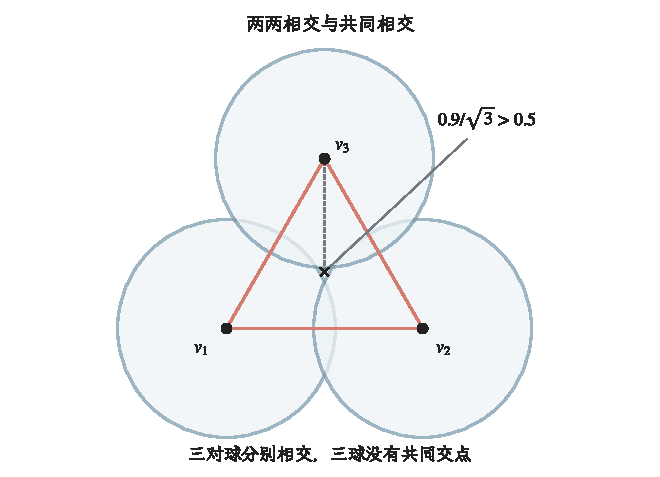
\includegraphics[width=\linewidth]{figures/01-mathematical-preliminaries/02-linear-algebra-and-geometry/matplotlib/teaching-linear-probability/geometry-cech-rips-intersection.pdf}
 \caption{固定同组三点比较共同交集与成对条件。正三角形边长$0.9$，
 $\varepsilon=1$，蓝色开球半径$0.5$；红色边满足两种构造的连边条件。
 三球无共同交点，Čech不含二维面，Rips含二维面。
 中心到各顶点的距离为$0.9/\sqrt3>0.5$。圆周只标开球边界，图为解析教学构造。}
 \label{fig:geometry-cech-rips-intersection}
\end{figure}

尺度变化后仍可给出明确包含关系。对任意$\eta>0$，有
\[
 \mathcal C_\varepsilon\subseteq\mathcal R_\varepsilon
 \subseteq\mathcal C_{2\varepsilon+\eta}.
\]
第一个包含关系由共同交点和三角不等式推出。
对第二个，任选一个顶点作候选共同交点，它到其余顶点的距离至多$\varepsilon$，
严格小于新球半径$\varepsilon+\eta/2$。
若全部球改用闭球，在相应定义下可取尺度常数$2$而不加$\eta$。
这些是足够的普适常数，不声称最紧；同一尺度的复形仍不能互换。

复形何时能代表球并集的拓扑，还依赖覆盖条件。良好覆盖（good cover）要求每个
非空有限交集都可连续收缩到一点；有限欧氏开球的交集为凸集，满足这项要求。
神经引理（nerve lemma）在该条件下说明Čech复形与球并集同伦等价，即二者存在相互映射，
来回复合可以连续变形到恒等映射。这里不要求两映射互为逆，所以比同胚弱：
闭区间可连续收缩到一个点，与单点空间同伦等价，却不可能与它存在双射。
这个结论不等于球并集已经恢复了未知潜在流形；
后者还需要采样覆盖和尺度条件。

为计算未被填充的环，需要把端点抵消与高阶填充分别记录。
选定顶点次序后，以$[v_0,\ldots,v_k]$表示有向单纯形，交换两顶点使符号反转。
有向$k$维单纯形的实系数线性组合称为$k$维链，
组成向量空间$C_k(\mathcal K;\mathbb R)$。边界算子读取每个面的有向边缘：
\begin{equation}
 \partial_k[v_0,\ldots,v_k]
 =\sum_{i=0}^k(-1)^i[v_0,\ldots,\widehat{v_i},\ldots,v_k],
 \qquad k\geq1,
 \label{eq:geometry-simplicial-boundary}
\end{equation}
尖帽表示删去该顶点，算子线性延伸到全部链。
本章采用非约化同调，约定$C_{-1}=\{0\}$、$\partial_0=0$。
例如$\partial_1[1,2]=[2]-[1]$，端点的正负表示方向。

\begin{lemma}[边界的边界为零]
\label{lem:geometry-boundary-squared-zero}
上述算子满足
\begin{equation}
 \partial_{k-1}\partial_k=0,\qquad k\geq1.
 \label{eq:geometry-boundary-squared-zero}
\end{equation}
\end{lemma}
\begin{proof}
$k=1$时由$\partial_0=0$成立。对$k\geq2$，固定$i<j$，
两次删除$v_i,v_j$后得到相同的$(k-2)$维面。
先删$i$再删原来的$j$，系数为$(-1)^i(-1)^{j-1}$；
先删$j$再删$i$，系数为$(-1)^j(-1)^i$，两者相反。
所有项都按这样的顶点对成对抵消，因此结论对基单纯形成立；
由线性性，对全部链成立。
\end{proof}

边界必定闭合，但闭合的圈未必由复形中的某个面填充。
这正好可以用上一章的核、像与商空间表达。
\begin{definition}[闭链、边界与同调空间]
\label{def:geometry-homology-space}
满足$\partial_kc=0$的链称为\term{闭链}（cycle），
能写成$c=\partial_{k+1}b$的链称为\term{边界}（boundary）。
由$\partial_k\partial_{k+1}=0$，有
$\operatorname{im}\partial_{k+1}\subseteq\ker\partial_k$。
实系数\term{同调空间}（homology space）及其维数定义为
\[
 H_k(\mathcal K;\mathbb R)=\ker\partial_k/\operatorname{im}\partial_{k+1},
 \qquad \beta_k=\dim H_k(\mathcal K;\mathbb R).
\]
$\beta_k$称为第$k$个\term{Betti数}（Betti number）。
\end{definition}
商空间沿用定义~\ref{def:linear-algebra-quotient-space}：
两个闭链相差一个边界时被视为同类。因而$H_k$保留的不是全部闭链，
而是无法用已有高阶填充消去的部分；$\beta_0$计算连通分支，
$\beta_1$计算实系数意义下独立的一维环。

取
$\mathcal K_{\mathrm{loop}}
=\{\{1\},\{2\},\{3\},\{1,2\},\{2,3\},\{1,3\}\}$。
链$c=[1,2]+[2,3]-[1,3]$的端点逐一抵消，故$\partial_1c=0$。
$\partial_1$的秩为$2$，一维闭链空间维数为$3-2=1$，
而没有二维面，故$\beta_1=1$、$\beta_0=3-2=1$。
加入$[1,2,3]$后，$c=\partial_2[1,2,3]$成为边界，$\beta_1$降为$0$；
$\partial_1$不变，所以$\beta_0$仍为$1$。
图~\ref{fig:geometry-cycle-filled-simplex}只改变面集合，顶点与边保持相同。
\begin{figure}[htbp]
 \centering
 % Two finite simplicial complexes with the same vertices and edges.
% Intended canvas: 112 mm by 36 mm. Exact combinatorial teaching construction.
\begin{tikzpicture}[x=1cm,y=1cm,font=\figurefont\small,text=FigureInk,
  line width=1.1pt,draw=FigureStroke]
 \path[use as bounding box] (0,0) rectangle (11.2,3.6);
 \begin{scope}[shift={(1.3,0.75)}]
  \coordinate (a) at (0,0); \coordinate (b) at (2.4,0);
  \coordinate (c) at (1.2,1.75);
  \draw (a)--(b)--(c)--cycle;
  \foreach \v in {a,b,c} \fill[FigureInk] (\v) circle (1.3pt);
  \node[below] at (a) {$1$}; \node[below] at (b) {$2$};
  \node[above] at (c) {$3$};
  \node at (1.2,2.5) {空心三角环};
  \node at (1.2,-0.55) {$\beta_1=1$};
 \end{scope}
 \begin{scope}[shift={(7.0,0.75)}]
  \coordinate (a) at (0,0); \coordinate (b) at (2.4,0);
  \coordinate (c) at (1.2,1.75);
  \fill[FigureYellowFill] (a)--(b)--(c)--cycle;
  \draw (a)--(b)--(c)--cycle;
  \foreach \v in {a,b,c} \fill[FigureInk] (\v) circle (1.3pt);
  \node[below] at (a) {$1$}; \node[below] at (b) {$2$};
  \node[above] at (c) {$3$};
  \node at (1.2,2.5) {填充三角面};
  \node at (1.2,-0.55) {$\beta_1=0$};
 \end{scope}
\end{tikzpicture}%

 \caption{一圈边是否已填充，取决于高阶面而非边图。左侧闭链
 $c=[1,2]+[2,3]-[1,3]$不是边界；右侧加入$[1,2,3]$后有
 $c=\partial_2[1,2,3]$。两者$\beta_0=1$，$\beta_1$分别为$1$与$0$。
 图为组合教学示例，不代表某个观测点云的真实拓扑。}
 \label{fig:geometry-cycle-filled-simplex}
\end{figure}

复形的规模还依赖邻域尺度。开带$\mathcal M_{\mathrm{strip}}$与开矩形同胚，
中心线$\mathcal C$与开区间同胚，都没有全局环。
闭合中心线得到圆，保留横向自由度并闭合则得到二维环带；
维数不同，但都保留绕中心的一维环。只有在采样和尺度适当时，样本复形才有理由
反映这些区别。尺度太小会把采样空隙误认作分支；太大则可能跨折连边，
并以高阶面填掉原来的环。

单一尺度可能把采样空隙当成孔洞，也可能把真实孔洞填平。持续同调（persistent homology）
因此跟踪尺度逐渐增大时，同调类何时出现、何时消失。存在于较宽尺度范围内的结构
提供了跨尺度信息，但仍不能仅凭持续时间就认定它对应任务中的真实结构。
若$N_k$是$k$维单纯形数，Euler示性数
$\chi=\sum_k(-1)^kN_k$是更粗的摘要：空心三角形为$3-3=0$，
填充三角形为$3-3+1=1$。由秩--零度关系
$N_k=\beta_k+\operatorname{rank}\partial_k+\operatorname{rank}\partial_{k+1}$，
交替求和后中间秩抵消，也得到$\chi=\sum_k(-1)^k\beta_k$。
不同Betti数组甚至不同拓扑都可能有同一个$\chi$，一个标量不足以代替分别分析。

用硬阈值连边时，两点距离只要稍微超过阈值，就会从相连突然变成不相连。为了记录
接近程度，可以改用软关系，以$\mu_{i,j}\in[0,1]$表示所选局部尺度下的连接强度；
这只是隶属度，不自动是事件概率。高阶强度例如可取全部边强度的最小值，
但必须声明采用哪种规则。一种常见的合并运算是
\begin{equation}
 a\mathbin{\sqcup}b=a+b-ab=1-(1-a)(1-b),\qquad a,b\in[0,1].
 \label{eq:geometry-fuzzy-union}
\end{equation}
结果仍在$[0,1]$内；交换性由对称式给出，结合性由
$1-(1-a)(1-b)(1-c)$给出，$0$为恒等元，任一输入为$1$时输出为$1$。
这些性质使它成为明确定义的软并集，却没有提供独立事件的随机试验或联合分布。
核权重、相似度、置信度与概率的校准要求不能仅凭数值范围混同。

UMAP等方法由局部距离构造带强度的关系，再优化低维坐标以匹配这些关系；
具体目标与优化过程留给
\BookChapterRef{chap:dimensionality-reduction}{第三卷“模型”的“降维”章}。
低维图像中的分离簇或孔洞还可能受邻居数、尺度、初始化与优化误差影响。
拓扑方法不能修复错误的局部输入：跨折捷径会被忠实组合，完全漏采的区域也无法凭空
恢复。采样覆盖、局部关系与尺度共同限制结论。

局部坐标之间的过渡只有在区域衔接时才能复合。若要统一记录这种“有起点和终点的
变换”，可以使用\term{范畴}（category）：
它包含对象、对象之间的箭头及各对象的恒等箭头，
仅在端点匹配时复合箭头，复合满足结合律与恒等律。
函子（functor）把对象和箭头映到另一范畴，同时保持恒等与复合。
例如坐标区域间可复合的过渡可按这种方式记录。
这只是组合表示的延伸语言，本章的距离与同调推导均不依赖它，
也不因引入这些名称获得额外的恢复保证。

\section{非线性空间的局部线性化}
\label{sec:geometry-manifold-local-linearization}

坐标图记录位置，却还没有说明从当前位置可以怎样动。以下固定光滑流形模型，
以局部参数化计算真实的一阶方向，再讨论只有样本时怎样估计这些方向。
解析模型与样本估计解决同一个局部问题，但它们的输入与保证不同。

\subsection{已知参数化下的局部线性化}
\label{sec:geometry-analytic-local-linearization}

从$\bm p=\varphi(\bm z)$出发，坐标变化$\bm v$经Jacobian
$\bm J_\varphi(\bm z)$映为环境空间中的瞬时速度。
\term{切空间}（tangent space）收集所有这样的可行速度；
它描述一阶方向，并不是可行集合本身的一小块。

\begin{definition}[嵌入流形的切空间]
\label{def:geometry-tangent-space}
设$\varphi:U\subseteq\mathbb R^d\to\mathcal M\subseteq\mathbb R^D$
是局部参数化，$\bm p=\varphi(\bm z)$。定义
\begin{equation}
 T_{\bm p}\mathcal M
 =\{\bm J_\varphi(\bm z)\bm v:\bm v\in\mathbb R^d\}.
 \label{eq:geometry-tangent-space-chart}
\end{equation}
\end{definition}
Jacobian列满秩保证这是$d$维向量空间，其原点是零速度。
画在$\bm p$旁边的仿射切平面则是$\bm p+T_{\bm p}\mathcal M$；
点的位置与速度向量的零点不能混为一谈。

\begin{lemma}[曲线速度与坐标刻画相容]
\label{lem:geometry-tangent-curves}
$T_{\bm p}\mathcal M$恰是全部光滑曲线
$\gamma:(-\epsilon,\epsilon)\to\mathcal M$、$\gamma(0)=\bm p$
的速度$\gamma'(0)$组成的集合，并且与局部坐标选择无关。
\end{lemma}
\begin{proof}
在足够小的参数区间内，曲线落入当前坐标图，写成
$\gamma(t)=\varphi(\bm z(t))$。链式法则给出
$\gamma'(0)=\bm J_\varphi(\bm z)\bm z'(0)$，故每个曲线速度都属于所定义的空间。
反过来，任意$\bm v\in\mathbb R^d$给出曲线
$t\mapsto\varphi(\bm z+t\bm v)$；因为$U$开，足够小的$t$仍在定义域内，
其初速度为$\bm J_\varphi(\bm z)\bm v$。

若另一参数化满足$\widetilde\varphi=\varphi\circ\psi$，
坐标过渡$\psi$的Jacobian可逆，且
$\bm J_{\widetilde\varphi}=\bm J_\varphi\bm J_\psi$。
右乘可逆矩阵不改变值域，两张图因而给出同一切空间。
\end{proof}

在点带中直接求导，可核对两个自由度：
\begin{align}
 \frac{\partial\Phi}{\partial s}
 &=\left(1+\frac uR\right)
   \begin{bmatrix}-\sin(s/R)\\\cos(s/R)\end{bmatrix},
 \label{eq:geometry-strip-s-tangent}\\
 \frac{\partial\Phi}{\partial u}
 &=\begin{bmatrix}\cos(s/R)\\\sin(s/R)\end{bmatrix}.
 \label{eq:geometry-strip-u-tangent}
\end{align}
因$|u|<w<R$，第一列不为零，两列正交且线性无关；
开带的切空间是整个$\mathbb R^2$。中心线则只允许$u=0$，
\[
 T_{\Phi(s,0)}\mathcal C
 =\operatorname{span}\{(-\sin(s/R),\cos(s/R))^\top\}.
\]
径向方向对开带可行，对中心线不可行。中心线的切线随位置转动，
没有一条固定线性子空间等于各处的切空间。

图~\ref{fig:geometry-strip-tangent-coordinates}上半部把切向速度画在点旁，
下半部比较同一坐标增量对应的实际弧长。方向数目决定局部维数，
坐标增量怎样换算为长度则留待度量处理。
\begin{figure}[htbp]
 \centering
 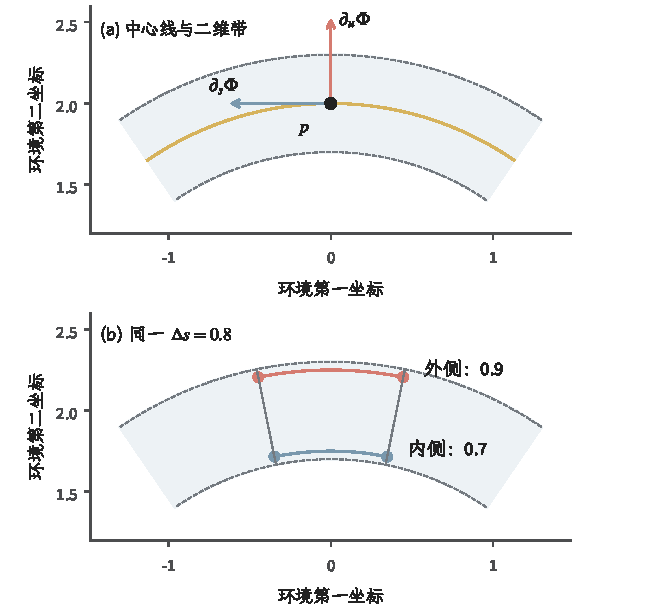
\includegraphics[width=\linewidth]{figures/01-mathematical-preliminaries/02-linear-algebra-and-geometry/matplotlib/concepts-linear-geometry/geometry-strip-tangent-coordinates.pdf}
 \caption{开带与中心线的局部方向不同。取$R=2$、$w=0.3$。
 上图的两个参数方向属于二维开带，仅以中心线为对象时，径向方向不属于其切空间；
 箭头平移到$\bm p$只是画法。下图取$u=-0.25,0.25$，同一$\Delta s=0.8$
 对应圆弧长度$0.7,0.9$。灰虚线为不纳入开带的边界，两图等比例绘制，均为解析教学示例。}
 \label{fig:geometry-strip-tangent-coordinates}
\end{figure}

切空间之所以适合近似，由Taylor展开说明。若参数化在当前邻域内二阶导数有界，则
\begin{equation}
 \varphi(\bm z+\bm h)-\varphi(\bm z)
 =\bm J_\varphi(\bm z)\bm h+O(\lVert\bm h\rVert_2^2).
 \label{eq:geometry-manifold-local-taylor}
\end{equation}
一阶项属于切空间，故环境位移投到法向正交补后只剩二阶余项。
这是局部结论，常数依赖所选邻域及二阶导数界；不能将它延伸到任意大步长。
法向偏离反映嵌入在环境中怎样弯曲，不等于后文要定义的内在曲率。
在二维开带中法向空间为零，弯曲坐标线本身就不构成法向误差。

若流形由约束$F(\bm x)=\bm0$给出，其中
$F:\mathbb R^D\to\mathbb R^{D-d}$在$\bm p$附近光滑且
$\bm J_F(\bm p)$行满秩，就能选出$D-d$列组成可逆方阵。
重排坐标后，定理~\ref{thm:analysis-implicit-function}把这$D-d$个变量
解为其余$d$个变量的光滑函数，后者便给出局部参数化。
对约束内曲线求导得$\bm J_F(\bm p)\gamma'(0)=\bm0$；
所以切空间包含于该矩阵的核。参数化给出$d$维切空间，
秩--零度关系又说明核为$d$维，故$T_{\bm p}\mathcal M=\ker\bm J_F(\bm p)$。
满秩条件不能省略：$F(x,y)=x^2+y^2$在原点导数为零，
核是整个平面，但零水平集只有一个点，真实可行速度只有零向量。

不仅位置可被映射，位置变化也需要随映射传递。
设$F:\mathcal M\to\mathcal N$，其坐标表达
$\psi^{-1}\circ F\circ\varphi$光滑，则称$F$光滑。
它在$\bm p$处的微分（differential）把输入速度转成输出速度：
\[
 \mathrm dF_{\bm p}(\bm v)
 =\left.\frac{\mathrm d}{\mathrm dt}F(\gamma(t))\right|_{t=0},
 \qquad\gamma(0)=\bm p,\quad\gamma'(0)=\bm v.
\]
若$\bm v=\bm J_\varphi(\bm z)\bm a$，令
$\bm w=\psi^{-1}(F(\bm p))$，则
\begin{equation}
 \mathrm dF_{\bm p}(\bm v)
 =\bm J_\psi(\bm w)
   \bm J_{\psi^{-1}\circ F\circ\varphi}(\bm z)\bm a.
 \label{eq:geometry-map-differential}
\end{equation}
右端只依赖初速度，不依赖实现速度的曲线，因此定义良好且线性。
坐标变换时两侧的Jacobian因链式法则相互抵消；
$\mathrm dF_{\bm p}:T_{\bm p}\mathcal M\to T_{F(\bm p)}\mathcal N$
是几何映射，矩阵只是其坐标记录。复合还满足
$\mathrm d(H\circ F)_{\bm p}=\mathrm dH_{F(\bm p)}\circ\mathrm dF_{\bm p}$。

对标量函数$f:\mathcal M\to\mathbb R$，微分读取速度引起的一阶数值变化。
\term{余切空间}（cotangent space）$T_{\bm p}^*\mathcal M$就是
$T_{\bm p}\mathcal M$的线性泛函空间，泛函的含义沿用
定义~\ref{def:functional-bounded-linear-functional}。
有限维向量空间上的全部线性读取组成其对偶空间（dual space）；
所以$\mathrm df_{\bm p}\in T_{\bm p}^*\mathcal M$，不是一个切向量。
写局部坐标为$(z^1,\ldots,z^d)$时，上标在这里是坐标编号而非迭代次数。
坐标切基为$\partial_i=\partial\varphi/\partial z^i$，
其对偶基$\mathrm dz^i$满足$\mathrm dz^i(\partial_j)=\delta_{i,j}$，
也就是$\mathrm dz^i(\sum_j a^j\partial_j)=a^i$：它读出速度的第$i$个坐标系数。于是
\[
 \mathrm df=\sum_i\partial_i(f\circ\varphi)\,\mathrm dz^i,\qquad
 \mathrm df\!\left(\sum_i a^i\partial_i\right)
 =\sum_i\partial_i(f\circ\varphi)a^i.
\]
例如圆上$f(\cos\theta,\sin\theta)=\cos\theta$，
角速度$a$对应的数值变化为$-a\sin\theta$。
要把这个线性读取规则表示成“最陡方向”，还须指定方向长度，
所以梯度将在度量建立后定义。

\subsection{观测样本下的局部线性化}
\label{sec:geometry-sampled-local-linearization}

只有$\bm x_i=\bm p_i+\bm\epsilon_i$时，参数化与潜在位置通常未知。
我们可以考察附近样本主要沿哪些方向变化，用这些方向近似真实切空间。局部PCA
（local principal component analysis）就是按这个思路，在小邻域中寻找主要的线性
变化方向。它估计一个已经选定的流形模型，并不定义流形本身。
必须先说明潜在对象是二维带还是一维中心线，才能确定希望估计什么。

给观测$\bm x_i$选择邻居索引集$N_i$和权重
$\alpha_{i,j}\geq0$、$\sum_{j\in N_i}\alpha_{i,j}=1$，计算
\begin{equation}
 \overline{\bm x}_i=\sum_{j\in N_i}\alpha_{i,j}\bm x_j,\qquad
 \bm C_i=\sum_{j\in N_i}\alpha_{i,j}
  (\bm x_j-\overline{\bm x}_i)(\bm x_j-\overline{\bm x}_i)^\top.
 \label{eq:geometry-local-weighted-covariance}
\end{equation}
若潜在维数$d$给定，取$\bm C_i$最大$d$个特征值对应的正交特征向量
$\widehat{\bm U}_i$，其列空间$\widehat T_i$为估计方向子空间。
若$d$未知，需另由谱和误差模型判断；不能把预先指定的特征向量数当成维数发现。
局部均值消去样本位置偏移，但不保证等于$\bm p_i$。

计算结果要与真实对象分开。$T_{\bm p_i}\mathcal M$是潜在位置处的真实方向空间，
$\widehat T_i$是从样本估计出的方向空间，二者都以零速度为原点。把估计方向空间
平移到$\overline{\bm x}_i$或$\bm x_i$处，才得到图中画出的仿射切平面近似。
若$d<D$，一般环境噪声使$\bm x_i\notin\mathcal M$，
此时$T_{\bm x_i}\mathcal M$甚至没有定义。
二维开带是当前例外：小噪声下观测仍在开带内，其切空间仍为$\mathbb R^2$，
但这不表示已经识别出生成它的潜在位置。

式~\eqref{eq:geometry-manifold-local-taylor}解释了误差来源。
在正则局部坐标中，邻域尺度为$h$时，切向位移通常为$O(h)$，
嵌入法向偏离为$O(h^2)$。若采样在各切方向上充分展开，
切向协方差特征值具有$h^2$量级；法向位移的平方贡献则可达到$h^4$量级。
这些尺度比较需要二阶导数有界和非退化局部采样，单靠光滑性并不保证谱间隙。

上一章的子空间扰动结论可用于把误差变成方向误差：
若理想局部协方差在第$d$与第$d+1$特征值间有间隙$\delta>0$，
而观测造成的算子范数扰动相对$\delta$足够小，则估计子空间的偏转受
$\lVert\bm E\rVert_2/\delta$控制。这里$\bm E$要包括有限样本波动、
噪声、邻域错选及非线性近似误差，不能只代入测量噪声方差。

缩小邻域会降低法向二阶偏差，却减少样本并压低真实信号的谱尺度；
固定噪声不会随之自动消失。邻域过大时，中心线不同位置的切线已经明显转动，
PCA会把这些不同方向合在一起，结果未必接近中心点的切线。对二维窄带，若样本的横向覆盖不足或宽度小于噪声尺度，
第二个方向可能难以稳定识别，但潜在对象并不因此变成一维。
固定近邻数也不能解决非均匀密度带来的变化：稀疏处覆盖范围大，稠密处范围小。
潜在对象、采样密度、嵌入弯曲、邻域尺度、谱间隙和噪声必须一起解释。

即使局部方向估计准确，也尚未得到全局坐标。圆的每个邻域只有一个切方向，
却不能以单张无断点实坐标图覆盖。局部PCA提供的是后续几何计算的局部输入，
不是全局展开或任务语义正确性的保证。

\section{流形上相同切空间下的度量、距离与运动}
\label{sec:geometry-metric-path-geodesic}

这里每次比较的两个向量，都属于同一个点处的切空间。
沿路径时，速度可以属于随位置变化的切空间；计算长度只需在每个位置读出一个标量速度，
再把这些标量累计起来，不需要先把不同位置的向量搬到一起。

\subsection{同一点处的切向量度量}
\label{sec:geometry-same-point-metric}

切空间说明方向可不可行，却没有规定一单位坐标变化有多长。
点带外侧与内侧相同的$\mathrm ds$对应不同弧长，因而内积必须按位置指定。
\term{Riemann度量}（Riemannian metric）为每个切空间提供这种长度与夹角规则。

\begin{definition}[Riemann度量]
\label{def:geometry-riemannian-metric}
光滑流形$\mathcal M$上的Riemann度量$g$为每个$\bm p$指定内积
$g_{\bm p}:T_{\bm p}\mathcal M\times T_{\bm p}\mathcal M\to\mathbb R$，
且在任一光滑坐标切基$\partial_i$中，矩阵
$\bm G(\bm z)=[g_{i,j}(\bm z)]$、$g_{i,j}=g(\partial_i,\partial_j)$
的条目光滑。每个$\bm G$都对称正定。
\end{definition}
对同点切向量$\bm v,\bm w$，长度为
$\lVert\bm v\rVert_g=\sqrt{g_{\bm p}(\bm v,\bm v)}$；
非零时夹角满足
$\cos\vartheta=g_{\bm p}(\bm v,\bm w)/
(\lVert\bm v\rVert_g\lVert\bm w\rVert_g)$。
若它们的坐标分量为$\bm a,\bm b$，内积是$\bm a^\top\bm G\bm b$。
$\bm G$既不是样本协方差，也不必是全空间共享的常矩阵。

嵌入流形可以限制环境欧氏内积，得到诱导度量：
\begin{equation}
 \bm G(\bm z)=\bm J_\varphi(\bm z)^\top\bm J_\varphi(\bm z).
 \label{eq:geometry-induced-metric}
\end{equation}
对非零$\bm a$，满列秩保证
$\bm a^\top\bm G\bm a=\lVert\bm J_\varphi\bm a\rVert_2^2>0$。
若Jacobian退化，只会得到半正定形式；这不符合当前坐标中的Riemann度量条件。
也可以另选光滑正定内积，但这样会改变几何，而不只是改写坐标。

若旧坐标$\bm z=\psi(\bm v)$，记可逆Jacobian为$\bm A=\bm J_\psi$，
同一几何向量的旧分量等于$\bm A$乘新分量，所以
\begin{equation}
 \widetilde{\bm G}(\bm v)=
 \bm A^\top\bm G(\psi(\bm v))\bm A.
 \label{eq:geometry-metric-coordinate-transform}
\end{equation}
因此$\bm a^\top\widetilde{\bm G}\bm b
=(\bm A\bm a)^\top\bm G(\bm A\bm b)$。
改变分量而不改变度量会改变所计算的长度；按此式一起变换则仍描述同一内积。

点带的两个参数方向已在式~\eqref{eq:geometry-strip-s-tangent}与
\eqref{eq:geometry-strip-u-tangent}中求出，故
\begin{equation}
 \bm G(s,u)=
 \begin{bmatrix}(1+u/R)^2&0\\0&1\end{bmatrix}.
 \label{eq:geometry-strip-metric}
\end{equation}
横向速度$\dot u$的长度系数为$1$，纵向速度$\dot s$的系数为$1+u/R$。
在$R=2$、$u=\pm0.25$时，同一$\Delta s=0.8$沿固定$u$的圆弧
分别产生$0.9$与$0.7$的长度，与图~\ref{fig:geometry-strip-tangent-coordinates}一致。
内积权重来自坐标尺度，并不由该位置采到了多少点决定。

\subsection{沿路径的速度与长度}
\label{sec:geometry-path-speed-length}

设分段光滑路径$\gamma:[a,b]\to\mathcal M$在一张图中写成
$\gamma(t)=\varphi(\bm z(t))$。链式法则保证
$\dot\gamma(t)\in T_{\gamma(t)}\mathcal M$，度量读出的平方速度为
\begin{equation}
 \lVert\dot\gamma(t)\rVert_g^2
 =\dot{\bm z}(t)^\top\bm G(\bm z(t))\dot{\bm z}(t).
 \label{eq:geometry-riemannian-speed}
\end{equation}
将标量速度按时间累计，定义路径长度
\begin{equation}
 L_g(\gamma)=\int_a^b
 \sqrt{\dot{\bm z}(t)^\top\bm G(\bm z(t))\dot{\bm z}(t)}\,\mathrm dt.
 \label{eq:geometry-riemannian-curve-length}
\end{equation}
整条路径不在同一张图时，将紧区间$[a,b]$分成有限段，使每段落入一张图，
再求长度之和。紧致的路径像和坐标开覆盖保证能作这种有限分段。

这种计算不依赖坐标。在$\bm z=\psi(\bm v)$下，
$\dot{\bm z}=\bm A\dot{\bm v}$，
式~\eqref{eq:geometry-metric-coordinate-transform}给出
$\dot{\bm v}^\top\widetilde{\bm G}\dot{\bm v}
=\dot{\bm z}^\top\bm G\dot{\bm z}$。
每段被积的标量相同，所以重叠区域选哪张图、怎样进一步细分都不改变长度。

长度也不依赖沿同一路线前进的快慢。对保持方向的光滑重参数化$t=\tau(r)$，
新速度为$\dot\gamma(\tau(r))\tau'(r)$，
其长度因子为$|\tau'(r)|$；当$\tau'>0$时，
积分换元$\mathrm dt=\tau'(r)\mathrm dr$给出相同总长。
反向的光滑单调参数化配合积分端点互换也不改变长度。
允许停顿的分段正则重参数化可分段处理；来回多走则改变路线的经过次数，
不属于仅仅换速度。

瞬时切向可行不等于环境直线可行。单位圆上
$\bm p=(1,0)^\top$、$\bm v=(0,1)^\top\in T_{\bm p}\mathbb S^1$，
但$\lVert\bm p+t\bm v\rVert_2=\sqrt{1+t^2}>1$对$t\neq0$成立。
速度只描述路径的一阶变化，保持有限步可行仍需在曲面上构造完整路径或更新映射。

\subsection{固定端点间的测地距离与近似}
\label{sec:geometry-endpoint-distance}

路径长度评价一条已经给出的路线。端点固定而路线可选时，要比较所有允许的路线；
完整空间已知和只有有限采样是这个问题的两种信息条件。

\subsubsection{连续空间下的测地距离}
\label{sec:geometry-continuous-geodesic-distance}

\begin{definition}[测地距离]
\label{def:geometry-geodesic-distance}
在Riemann流形$(\mathcal M,g)$的同一路径连通分支内，定义
\term{测地距离}（geodesic distance）为连接两点的全部分段光滑路径长度的下确界：
\begin{equation}
 d_g(\bm p,\bm q)=
 \inf_{\substack{\gamma(a)=\bm p\\\gamma(b)=\bm q}}L_g(\gamma).
 \label{eq:geometry-geodesic-distance}
\end{equation}
若无连接路径，约定值为$+\infty$；在可能不连通的整个空间上，它是扩展距离。
\end{definition}
这里的定义尚不要求存在最短路径，更不依赖测地线方程。
反向路径给出对称性，拼接两条近似最短路径给出三角不等式。
在一个足够小的坐标邻域内，按度量计算的向量长度，可以用其坐标向量的欧氏长度
乘以两个固定正常数从上下控制。这保证不同点之间的路程不能趋于零，因而每个
连通分支中确实得到度量。

对于欧氏诱导度量，由
$\bm q-\bm p=\int_a^b\dot\gamma(t)\,\mathrm dt$与三角不等式，
每条连接路径均满足$\lVert\bm q-\bm p\rVert_2\leq L_g(\gamma)$，
所以
\[
 \lVert\bm q-\bm p\rVert_2\leq d_g(\bm p,\bm q).
\]
若连接线段完全可行，就取等。反过来，只有下确界被允许路径达到时，
取等才迫使该最短路径沿线段行进，至多改变速度；
距离相等本身不保证线段可行。若换成任意非诱导度量，上述环境距离比较也不能照搬。

回到开中心线的两点$\bm p=\Phi(s,0)$、$\bm q=\Phi(t,0)$。
环境空间的弦长是
\begin{equation}
 \lVert\Phi(s,0)-\Phi(t,0)\rVert_2
 =2R\left|\sin\frac{s-t}{2R}\right|.
 \label{eq:geometry-strip-chord-distance}
\end{equation}
中心线以$s$为弧长参数，允许路径必须留在开弧内，因此
$d_{\mathcal C}(\bm p,\bm q)=|s-t|$。
二维带允许路径向内侧绕行，中心线弧只是候选，故
\[
 \lVert\bm p-\bm q\rVert_2
 \leq d_{\mathcal M_{\mathrm{strip}}}(\bm p,\bm q)
 \leq d_{\mathcal C}(\bm p,\bm q)=|s-t|.
\]
带宽、端点位置和允许域决定第二个不等式是否严格；
不能把这两种距离都称为不加区分的“沿带距离”。

另取完整单位圆作为独立例子。夹角$0\leq\theta\leq\pi$时，
允许选择短弧，内在距离为$\theta$，弦长为$2\sin(\theta/2)$。
在$\theta=\pi/2$时两者为$\pi/2$与$\sqrt2$；
小角度展开$2\sin(\theta/2)=\theta-\theta^3/24+O(\theta^5)$说明局部接近，
全局却不同。图~\ref{fig:geometry-circle-distances}在相同尺度上比较这两种量。
\begin{figure*}[htbp]
 \centering
 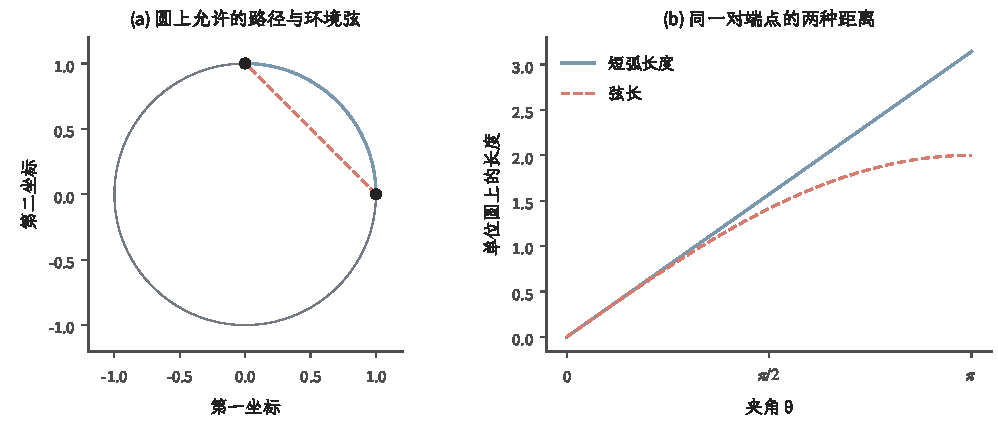
\includegraphics[width=\linewidth]{figures/01-mathematical-preliminaries/02-linear-algebra-and-geometry/matplotlib/analysis-geometry/geometry-circle-distances.pdf}
 \caption{完整单位圆的测地距离与环境弦长。左图夹角为$\pi/2$，
 蓝线为圆上的允许短弧，红虚线为穿过圆内的环境线段；
 右图比较$\theta\in[0,\pi]$时的两种长度。完整圆允许选择两段弧中的较短者，
 不能与开中心线或二维开带的允许路径混用。图为解析教学示例。}
 \label{fig:geometry-circle-distances}
\end{figure*}

为什么定义取下确界，而不直接取最小值？因为允许的路径未必包含一条最短路径。在穿孔平面
$\mathbb R^2\setminus\{\bm0\}$中，$(-1,0)^\top$与$(1,0)^\top$
之间可绕过任意小的圆孔，路径长度趋于$2$，却没有长度恰为$2$的允许路径。
哪些全局条件保证达到下确界，将在固定端点的最短路径问题中讨论。

\subsubsection{有限采样下的测地距离近似}
\label{sec:geometry-sampled-geodesic-distance}

只有观测点时，常把距离小于阈值$\varepsilon$的点相连，
或连接每个点的$k$个最近邻，再以$\lVert\bm x_i-\bm x_j\rVert_2$为边长。
一条边路径的长度是所经边长之和，最短边路径试图近似所选潜在流形上
$d_g(\bm p_i,\bm p_j)$。这里只借用顶点、边和路径的直观含义，
通用图算法留给第~\ref{part:discrete-mathematics-and-graph-theory}部分。

潜在对象必须先定。若观测不在潜在流形上，$d_g(\bm x_i,\bm x_j)$便未定义；
即使观测在二维开带内，也不能因此把它认作$\bm p_i$。
环境欧氏边长自然对应欧氏诱导度量的局部近似；
若目标采用另一个Riemann度量，就要据此修正边长，不能继续沿用欧氏弦长而声称目标未变。

邻域应足够小，使每条边只连接潜在流形上近似平直的一小段，避免把环境中靠得很近、
沿流形却相距很远的两段直接相连；
又要大到样本间的空隙能够连通。超过跨折环境间隔会引入捷径，低估沿潜在空间的距离；
小于采样空隙则会把一个真实分支拆开，返回无穷距离。
即使没有捷径，局部弦长误差与离散路径绕行误差也会共同作用，
不能无条件断言估计总在真实距离的同一侧。

固定$k$并不固定几何尺度。稀疏处第$k$个邻居可能很远，稠密处则很近，
有向近邻关系还可能不对称，需要声明如何对称化。
一致近似通常要求潜在流形光滑、采样在所研究区域逐渐稠密、
噪声相对邻域尺度受控，并让邻域半径随样本量缩小而仍足以覆盖采样空隙。
非紧开带若只在一部分采样，这些要求也只支持相应覆盖区域的结论。
具体收敛速度须结合采样分布与尺度选择证明，
最短边路径正确更不自动意味着后续全局坐标恢复正确。

\subsection{度量诱导的体积与积分}
\label{sec:geometry-riemannian-volume}

沿路径积分只覆盖一条路线。若要在整个曲面上累计函数值或变化量，就需要知道
每个小区域占多大面积；更高维时，相应的量是体积。
坐标切基围成的微小平行体，其平方体积是Gram行列式$\det\bm G$，
因此几何体积元为
\begin{equation}
 \mathrm dV_g=\sqrt{\det\bm G(\bm z)}\,\mathrm d\bm z.
 \label{eq:geometry-riemannian-volume}
\end{equation}
这是由度量产生的测度密度，不要求先为流形选定全局朝向。
一维时给出长度，二维时给出面积。

坐标变换$\bm z=\psi(\bm v)$下，
$\det\widetilde{\bm G}=(\det\bm A)^2\det\bm G$，所以
\[
 \sqrt{\det\widetilde{\bm G}}\,\mathrm d\bm v
 =\sqrt{\det\bm G(\psi(\bm v))}\,|\det\bm A|\,\mathrm d\bm v.
\]
它正是多元积分换元中的Jacobian因子，故对可积函数所得积分不依赖坐标。
跨图时必须避免把重叠区域重复计数，可分割成可测片段分别积分；
光滑计算也可使用从属于图册、和为$1$的局部权重来拼接。

点带中$\sqrt{\det\bm G}=1+u/R>0$，
小盒$\mathrm ds\,\mathrm du$在外侧对应较大面积。
中心线限制为$u=0$后的一维体积元是$\mathrm ds$，不是把二维面积直接代入。
若样本相对几何体积有密度$q$，其分布测度是$q\,\mathrm dV_g$；
简单样本平均近似该加权积分，并非自动近似$\int f\,\mathrm dV_g$。
几何体积与采样权重的差别将在离散平滑目标中再次出现。

当前开带无流形边界，但不是紧集。需要边界积分时，将另取有分片光滑边界的
截断闭域，并声明函数在边界的行为；不能只因图上画有虚线就把它当作同一个积分问题。

\section{流形上不同切空间的比较与曲率}
\label{sec:geometry-cross-point-comparison-curvature}

沿路径计算长度时，每个位置只输出一个标量。若要问速度有没有转弯，
或相邻两点的方向是否一致，就必须比较不同切空间中的向量。
即使流形嵌在同一个欧氏空间内，直接相减也可能产生法向分量：
圆上恒速运动的速度导数指向圆心，却没有沿圆加速。
需要把环境变化与流形内的方向变化分开。下面建立联络、测地运动和曲率，
所用的Riemann几何基础可参见Lee的教材\scite{math-lee2018riemannian}

\subsection{不同切空间的比较规则}
\label{sec:geometry-connection-comparison}

在每个位置指定一个可行方向，得到向量场。跨点比较规则应使其导数仍为切向量，
还应遵守加法和乘积求导；联络就是满足这些要求的微分规则。
它不是把所有切空间强行认成同一个空间，而是在局部说明怎样比较变化。

\begin{definition}[向量场与联络]
\label{def:geometry-connection}
光滑\term{向量场}（vector field）$\bm V$在每个$\bm p\in\mathcal M$选取
$\bm V(\bm p)\in T_{\bm p}\mathcal M$，其坐标分量光滑。
\term{联络}（connection）为两个光滑向量场$\bm U,\bm V$指定向量场
$\nabla_{\bm U}\bm V$，称为$\bm V$沿$\bm U$的
\term{协变导数}（covariant derivative），并满足
\[
 \begin{aligned}
 \nabla_{f\bm U+h\bm W}\bm V
   &=f\nabla_{\bm U}\bm V+h\nabla_{\bm W}\bm V,\\
 \nabla_{\bm U}(a\bm V+b\bm W)
   &=a\nabla_{\bm U}\bm V+b\nabla_{\bm U}\bm W,\\
 \nabla_{\bm U}(f\bm V)
   &=\bm U(f)\bm V+f\nabla_{\bm U}\bm V.
 \end{aligned}
\]
其中$f,h$为光滑函数，$a,b\in\mathbb R$，
$\bm U(f)=\mathrm df(\bm U)$为方向导数。
\end{definition}
第一条允许求导方向的系数是光滑函数，第二条只允许被求导向量场的系数是常数，
第三条说明为什么不能把第二条的常数任意换成光滑函数：
系数本身的变化必须保留。欧氏空间的普通方向导数满足这三项规则；
一般流形上，单独求坐标分量的导数不够，因为坐标切基本身也在变。

度量已经规定长度，新的导数应当与这一判断相容。
此外，非坐标方向场先后作用的顺序本来就可能不同，不能把这种差异误认为额外的几何扭转。
定义交换子$[\bm U,\bm V]$为对任意光滑$f$满足
\[
 [\bm U,\bm V](f)=\bm U(\bm V(f))-\bm V(\bm U(f))
\]
的向量场；在坐标基下，其第$k$个分量为
$\sum_i(U^i\partial_iV^k-V^i\partial_iU^k)$。
坐标方向$\partial_i,\partial_j$的交换子为零，一般方向场则未必。

\begin{example}[平面上不可交换的方向场]
\label{ex:geometry-plane-field-commutator}
在欧氏平面取$\bm U=\partial_x$、$\bm V=x\partial_y$。
$\bm U$始终沿$x$轴，$\bm V$沿$y$轴但其大小随$x$改变。
对任意光滑函数$f$，
\[
 \bm U(\bm V(f))=\partial_yf+x\partial_x\partial_yf,\qquad
 \bm V(\bm U(f))=x\partial_y\partial_xf,
\]
故$[\bm U,\bm V]=\partial_y$。先沿$x$方向移动，会改变随后沿$\bm V$移动的速度；
两个方向场的顺序差异在平面上就会出现。
欧氏空间的普通方向导数还给出
\[
 \nabla_{\bm U}\bm V=\partial_y,\qquad
 \nabla_{\bm V}\bm U=\bm0.
\]
二者之差恰是交换子。这个平坦例子说明，方向场本身随位置变化所产生的差异，
需要与几何结构额外产生的差异分开。
\end{example}

\begin{definition}[Levi--Civita联络]
\label{def:geometry-levi-civita-connection}
给定Riemann度量$g$，同时满足下列度量相容与无挠条件的联络，
称为它的\term{Levi--Civita联络}（Levi--Civita connection）：
\begin{align*}
 \bm U\bigl(g(\bm V,\bm W)\bigr)
 &=g(\nabla_{\bm U}\bm V,\bm W)+g(\bm V,\nabla_{\bm U}\bm W),\\
 \nabla_{\bm U}\bm V-\nabla_{\bm V}\bm U&=[\bm U,\bm V].
\end{align*}
\end{definition}
度量相容使内积的求导仍满足乘积法则；无挠规定联络在交换两个方向场时，
不产生交换子之外的差异。无挠\emph{不}声称
$\nabla_{\bm U}\nabla_{\bm V}\bm W
=\nabla_{\bm V}\nabla_{\bm U}\bm W$，后者涉及本节末尾的曲率。

每个光滑Riemann度量唯一确定这样的联络。其唯一性可以从两项条件直接看出：
轮换$\bm U,\bm V,\bm W$的度量相容等式，并用无挠条件消去交换项，得到
\begin{align}
 2g(\nabla_{\bm U}\bm V,\bm W)
 &=\bm U g(\bm V,\bm W)+\bm V g(\bm W,\bm U)
   -\bm W g(\bm U,\bm V)\notag\\
 &\quad+g([\bm U,\bm V],\bm W)-g([\bm V,\bm W],\bm U)
   +g([\bm W,\bm U],\bm V).
 \label{eq:geometry-koszul-formula}
\end{align}
右端只含已知度量、向量场和普通方向导数；正定性使其唯一确定
$\nabla_{\bm U}\bm V$。反过来，用此式定义该向量场，代入可检查联络的三条规则、
度量相容和无挠条件，因而也给出存在性。这个公式的用途是确定比较规则，
实际计算通常使用坐标系数或环境投影。

对继承欧氏度量的嵌入流形，设$\bm P_{\bm p}$为环境空间到
$T_{\bm p}\mathcal M$的正交投影，则
\begin{equation}
 \nabla_{\bm U}\bm V(\bm p)
 =\bm P_{\bm p}\,\mathrm d\bm V_{\bm p}(\bm U(\bm p)).
 \label{eq:geometry-projected-connection}
\end{equation}
这里把$\bm V$视为取值于环境$\mathbb R^D$的映射，先求环境导数再投影。
投影保持对切向量的内积，所以欧氏内积的乘积法则给出度量相容；
环境方向导数之差是已经切向的交换子，投影后仍不变，故也无挠。
由唯一性，这正是诱导度量的Levi--Civita联络。
若度量不是环境诱导度量，不能继续沿用这个欧氏正交投影公式。

\subsection{给定路径下的平行移动}
\label{sec:geometry-parallel-transport}

现在固定路径$\gamma(t)$和起点切向量，希望沿路保持方向。
“保持”不是要求环境坐标分量不变，而是要求联络测得的变化为零。
在坐标基中写
$\nabla_{\partial_i}\partial_j=\sum_k\Gamma^k_{i,j}\partial_k$，
则沿$\gamma(t)=\varphi(\bm z(t))$的向量
$\bm V(t)=\sum_jV^j(t)\partial_j$满足
\begin{equation}
 \frac{D\bm V}{\mathrm dt}
 =\sum_k\left(\dot V^k+
     \sum_{i,j}\Gamma^k_{i,j}(\bm z(t))\dot z^iV^j\right)\partial_k.
 \label{eq:geometry-covariant-derivative-along-path}
\end{equation}
第一项是分量变化，第二项修正坐标切基的变化；合起来才是坐标无关的协变导数。
对于欧氏诱导度量，式~\eqref{eq:geometry-projected-connection}沿路径写成
\[
 \frac{D\bm V}{\mathrm dt}
 =\bm P_{\gamma(t)}\frac{\mathrm d\bm V}{\mathrm dt},
\]
保留环境导数的切向部分。

\begin{definition}[平行移动]
\label{def:geometry-parallel-transport}
给定分段光滑路径$\gamma:[a,b]\to\mathcal M$和
$\bm v\in T_{\gamma(a)}\mathcal M$，沿路解
\[
 \frac{D\bm V}{\mathrm dt}=\bm0,\qquad \bm V(a)=\bm v.
\]
终值定义线性映射
$P_\gamma:T_{\gamma(a)}\mathcal M\to T_{\gamma(b)}\mathcal M$，
称为沿$\gamma$的\term{平行移动}（parallel transport）。
\end{definition}
坐标式是具有连续系数的线性常微分方程，初值唯一决定解；
沿有限段路径逐图求解并拼接即可，不要求流形完备。
反向路径给出逆映射，拼接路径对应映射复合。
对于Levi--Civita联络，
\[
 \frac{\mathrm d}{\mathrm dt}g(\bm V,\bm W)
 =g(D\bm V/\mathrm dt,\bm W)+g(\bm V,D\bm W/\mathrm dt)=0
\]
用于任意两个平行向量场。因此$P_\gamma$保持长度和夹角。
这个结论依赖度量相容，不能对任意联络直接宣称保距。

欧氏空间的直角坐标中$\Gamma^k_{i,j}=0$，平行移动保持向量的分量不变，
且与路径无关。球面则不同：向量必须始终切向，环境分量通常会改变，
不同路径的终值也可能不同。

\begin{example}[球面三段路径上的方向搬运]
\label{ex:geometry-sphere-parallel-transport}
在诱导度量的单位球面$\mathbb S^2$上，取
$N=(0,0,1)^\top$、$A=(1,0,0)^\top$、$B=(0,1,0)^\top$。
记三个坐标轴的单位向量为$\bm e_x,\bm e_y,\bm e_z$。
沿三条四分之一大圆弧$N\to A\to B\to N$搬运初始向量
$\bm V(N)=\bm e_x$。各段用$t\in[0,\pi/2]$参数化：
\[
 \begin{array}{c|c|c}
  \text{路径}&\gamma(t)&\bm V(t)\\ \hline
  N\to A&(\sin t,0,\cos t)^\top&(\cos t,0,-\sin t)^\top\\
  A\to B&(\cos t,\sin t,0)^\top&(0,0,-1)^\top\\
  B\to N&(0,\cos t,\sin t)^\top&(0,\sin t,-\cos t)^\top
 \end{array}
\]
每段都有$\gamma^\top\bm V=0$与$\lVert\bm V\rVert_2=1$。
第一段$\dot{\bm V}=-\gamma$，第二段$\dot{\bm V}=\bm0$，
第三段$\dot{\bm V}=\gamma$，环境导数全部是法向或零，投影后的协变导数为零。
两处接点的向量同为$-\bm e_z$，故三段连续拼接。
返回$N$时向量成为$\bm e_y$，与初始$\bm e_x$相差$\pi/2$。
若始终留在$N$，搬运则不改变向量，说明仅给起终点不能决定平行移动。
\end{example}

图~\ref{fig:geometry-sphere-parallel-transport}画出这些向量的沿路变化。
在$B\to N$段，向量与前进速度相反；保持方向不意味着向量必须指向前进方向。
\begin{figure}[htbp]
 \centering
 % Orthographic projection: x=(y-x)/sqrt(2), y=(2z-x-y)/sqrt(6).
% All tangent arrows have the same length before projection.
\begin{tikzpicture}[figure picture,x=1mm,y=1mm,
  transport/.style={draw=FigureRed,line width=.95pt,
    -{Stealth[length=1.8mm,width=1.2mm]}},
  route/.style={draw=FigureBlue,line width=1.1pt,
    -{Stealth[length=1.8mm,width=1.2mm]}},
  every node/.append style={fill=none,inner sep=1.2pt}]
 \path[use as bounding box] (0,10) rectangle (112,77);
 \begin{scope}[shift={(56,40)}]
  \draw[FigureGrid] (0,0) circle[radius=28];
  \draw[FigureGrid,dashed,samples=81,domain=135:315]
   plot ({28/sqrt(2)*(sin(\x)-cos(\x))},
         {-28/sqrt(6)*(cos(\x)+sin(\x))});
  \draw[FigureGrid,samples=81,domain=-45:135]
   plot ({28/sqrt(2)*(sin(\x)-cos(\x))},
         {-28/sqrt(6)*(cos(\x)+sin(\x))});
  \draw[route,samples=61,domain=0:90]
   plot ({-28/sqrt(2)*sin(\x)},
         {28/sqrt(6)*(2*cos(\x)-sin(\x))});
  \draw[route,samples=61,domain=0:90]
   plot ({28/sqrt(2)*(sin(\x)-cos(\x))},
         {-28/sqrt(6)*(cos(\x)+sin(\x))});
  \draw[route,samples=61,domain=0:90]
   plot ({28/sqrt(2)*cos(\x)},
         {28/sqrt(6)*(2*sin(\x)-cos(\x))});
  \foreach \t in {30,60} {
   \draw[transport]
    ({-28/sqrt(2)*sin(\t)},{28/sqrt(6)*(2*cos(\t)-sin(\t))})
    -- ++({-11/sqrt(2)*cos(\t)},
          {11/sqrt(6)*(-2*sin(\t)-cos(\t))});
   \draw[transport]
    ({28/sqrt(2)*(sin(\t)-cos(\t))},
     {-28/sqrt(6)*(cos(\t)+sin(\t))})
    -- ++(0,{-22/sqrt(6)});
   \draw[transport]
    ({28/sqrt(2)*cos(\t)},{28/sqrt(6)*(2*sin(\t)-cos(\t))})
    -- ++({11/sqrt(2)*sin(\t)},
          {11/sqrt(6)*(-2*cos(\t)-sin(\t))});
  }
  \coordinate (N) at (0,{56/sqrt(6)});
  \coordinate (A) at ({-28/sqrt(2)},{-28/sqrt(6)});
  \coordinate (B) at ({28/sqrt(2)},{-28/sqrt(6)});
  \draw[draw=FigureYellow,line width=1.2pt,
    -{Stealth[length=2mm,width=1.4mm]}]
    (N)--++({-11/sqrt(2)},{-11/sqrt(6)}) coordinate (Initial);
  \draw[transport] (N)--++({11/sqrt(2)},{-11/sqrt(6)})
    coordinate (Final);
  \foreach \p in {N,A,B} {\fill[FigureInk] (\p) circle[radius=.6];}
  \node[above] at (N) {$N$};
  \node[below left] at (A) {$A$};
  \node[below right] at (B) {$B$};
 \end{scope}
 \draw[FigureMuted,line width=.4pt] (Initial)--(36,70)--(26,70);
 \node[above] at (26,70) {初始 $\bm e_x$};
 \draw[FigureMuted,line width=.4pt] (Final)--(76,70)--(87,70);
 \node[above] at (87,70) {终值 $\bm e_y$};
\end{tikzpicture}

 \caption{单位球面上沿$N\to A\to B\to N$的平行移动。
 蓝色为给定的三条大圆弧，红箭头为例~\ref{ex:geometry-sphere-parallel-transport}
 中逐段计算的切向量。沿路协变导数为零，返回$N$后的方向却由黄色初始箭头
 $\bm e_x$变为红色终值箭头$\bm e_y$。
 箭头在三维中等长，投影到纸面后的长度可以不同。图为解析教学示例。}
 \label{fig:geometry-sphere-parallel-transport}
\end{figure}

这里的变换由路径和联络决定，不是任意选一个旋转来对齐环境向量。
前文群作用规定的是输入在指定变换下的响应；平行移动规定的是沿几何路径的方向比较，
即使二者有时都用矩阵表示，也不能据此互换。

\subsection{不同条件下的测地运动与最短路径}
\label{sec:geometry-geodesic-motion-minimization}

平行移动把路径当作输入、向量场当作未知量。若要求路径自己的速度平行移动，
路径也变成未知量。给定初速度时，这是运动方程的初值问题；
只给两个端点时，还要决定该沿哪条路径前进，最短性是额外的比较要求。

\subsubsection{初速度条件下的测地运动}
\label{sec:geometry-geodesic-initial-value}

\begin{definition}[测地线]
\label{def:geometry-geodesic}
相对于Riemann流形的Levi--Civita联络，采用仿射参数的曲线$\gamma$若满足
\[
 \frac{D\dot\gamma}{\mathrm dt}=\bm0,
\]
称为\term{测地线}（geodesic）。
\end{definition}
它没有切向加速度，速度沿自身路径作平行移动。
度量相容进一步给出
$\frac{\mathrm d}{\mathrm dt}\lVert\dot\gamma\rVert_g^2
=2g(D\dot\gamma/\mathrm dt,\dot\gamma)=0$，因此速度大小恒定。
环境加速度仍可非零，例如球面大圆需要法向加速度才能留在球面。

“仿射参数”说明换元$t=ar+b$、$a\neq0$保留这个方程。
一般换元则产生
\[
 \frac{D}{\mathrm dr}\frac{\mathrm d\gamma}{\mathrm dr}
 =(\tau'(r))^2\frac{D\dot\gamma}{\mathrm dt}
   +\tau''(r)\dot\gamma.
\]
非匀速参数化可以描出相同几何轨迹，却不再满足零协变加速度。
因此不能把路径长度的任意重参数化不变性照搬到这个运动方程。

要在坐标中求解，先用式~\eqref{eq:geometry-koszul-formula}取
$\bm U=\partial_i,\bm V=\partial_j,\bm W=\partial_\ell$。
坐标方向交换子为零，于是
\[
 2\sum_k g_{k,\ell}\Gamma^k_{i,j}
 =\partial_i g_{j,\ell}+\partial_j g_{i,\ell}-\partial_\ell g_{i,j}.
\]
乘逆度量便得到Christoffel符号
\begin{equation}
 \Gamma^k_{i,j}
 =\frac12\sum_{\ell=1}^d g^{k,\ell}
  \left(\frac{\partial g_{\ell,j}}{\partial z^i}
       +\frac{\partial g_{i,\ell}}{\partial z^j}
       -\frac{\partial g_{i,j}}{\partial z^\ell}\right),
 \qquad [g^{i,j}]=\bm G^{-1}.
 \label{eq:geometry-christoffel-symbols}
\end{equation}
将$\bm V=\dot\gamma=\sum_j\dot z^j\partial_j$代入
式~\eqref{eq:geometry-covariant-derivative-along-path}，测地条件成为
\begin{equation}
 \ddot z^k+\sum_{i,j=1}^d
 \Gamma^k_{i,j}(\bm z)\dot z^i\dot z^j=0.
 \label{eq:geometry-geodesic-equation}
\end{equation}
要判断这组系数是否表示点处的几何对象，需要区分几何张量与一张普通分量表。
这里的几何张量（geometric tensor）是点处、与坐标无关的多线性对象；
换基只对它的各个输入和输出作线性变换。因此，零分量表换基后仍为零。
Christoffel符号不满足这一规律。以正半轴的欧氏度量为例，
在坐标$x>0$中有$g_{x,x}=1$、$\Gamma^x_{x,x}=0$；
改用$x=e^u$后，$g_{u,u}=e^{2u}$，式~\eqref{eq:geometry-christoffel-symbols}给出
\[
 \Gamma^u_{u,u}=\frac12 e^{-2u}\frac{\mathrm d}{\mathrm du}e^{2u}=1.
\]
所以Christoffel符号是联络的坐标系数，不是张量。
基向量的变化与这些系数共同组成协变加速度，后者及所得曲线仍是几何对象。

有了这组坐标方程，就能由起点和初速度计算运动。光滑系数使这个二阶方程在给定
$\gamma(0)=\bm p$、$\dot\gamma(0)=\bm v$后具有局部唯一解，
并光滑依赖初值。这里“局部”同时限制时间和坐标覆盖范围；
可以换图延拓，但若路径有限时间离开流形，延拓就会失败。
开单位球内的欧氏直线从原点出发，以速度$2\bm e_1$前进，
在$t=1/2$时便到达不属于该流形的边界，不能默认解存在至$t=1$。

\begin{definition}[指数映射]
\label{def:geometry-exponential-map}
对给定$\bm p$，若初速度$\bm v$的测地线$\gamma_{\bm v}$存在至$t=1$，
定义
\[
 \operatorname{Exp}_{\bm p}(\bm v)=\gamma_{\bm v}(1).
\]
它称为$\bm p$处的\term{指数映射}（exponential map），
其定义域至少包含$T_{\bm p}\mathcal M$中零向量的一个邻域。
\end{definition}
初速度缩放对应时间缩放：
$\operatorname{Exp}_{\bm p}(t\bm v)=\gamma_{\bm v}(t)$，只在两边均有定义时使用。
因而$\operatorname{Exp}_{\bm p}(\bm0)=\bm p$且
$\mathrm d(\operatorname{Exp}_{\bm p})_{\bm0}=\operatorname{id}_{T_{\bm p}\mathcal M}$。
逆函数定理保证在足够小邻域中它是微分同胚；
这为用切向量表示附近点提供了一种局部方式，不保证全局一一对应。

单位球面上，$\bm v\perp\bm p$、$r=\lVert\bm v\rVert_2$时，
\begin{equation}
 \operatorname{Exp}_{\bm p}(\bm v)
 =\cos r\,\bm p+\frac{\sin r}{r}\bm v,
 \label{eq:geometry-sphere-exponential}
\end{equation}
$r=0$时按连续延拓取$\bm p$。
对应曲线$\gamma(t)=\cos(tr)\bm p+\sin(tr)\bm v/r$
满足$\lVert\gamma(t)\rVert_2=1$、初速度为$\bm v$，
且$\ddot\gamma=-r^2\gamma$为纯法向，所以确实解测地线方程。
所有方向上长度为$\pi$的初速度都到达对跖点$-\bm p$；
即使映射处处有定义，也未必全局单射。

\subsubsection{固定端点条件下的最短路径}
\label{sec:geometry-endpoint-minimizing-path}

现在给定$\bm p,\bm q$，要找一条长度真正等于
式~\eqref{eq:geometry-geodesic-distance}中下确界的路径。要说明最短路径为什么满足
测地线方程，可以先把长度问题转成更便于求导的能量问题。固定时间区间$[a,b]$，定义
\[
 E(\gamma)=\frac12\int_a^b\lVert\dot\gamma\rVert_g^2\,\mathrm dt.
\]
由Cauchy--Schwarz不等式，
$L_g(\gamma)^2\leq2(b-a)E(\gamma)$，等号恰对应几乎处处恒定的速度大小。
因此对可作匀速参数化的非退化路径，最小化长度可联系到固定时间的能量最小化；
能量本身却不具有长度那样的任意重参数化不变性。

在局部坐标中，Lagrange函数为
$\mathscr L(\bm z,\dot{\bm z})=\frac12\sum_{i,j}g_{i,j}(\bm z)\dot z^i\dot z^j$。
取光滑扰动$\bm h$，满足$\bm h(a)=\bm h(b)=\bm0$，并令
$\bm z_\varepsilon(t)=\bm z(t)+\varepsilon\bm h(t)$。
取足够小的$\varepsilon$使路径仍在坐标域内。
若$\varphi$为当前坐标的参数化，一阶变分就是把整条路径沿这个方向改变后，
能量关于扰动幅度的导数：
\[
 \delta E[\bm h]
 =\left.\frac{\mathrm d}{\mathrm d\varepsilon}
 E(\varphi\circ\bm z_\varepsilon)\right|_{\varepsilon=0}.
\]
对积分求导并分部积分，得到
\[
 \delta E[\bm h]
 =\int_a^b\sum_k\left(
 \frac{\partial\mathscr L}{\partial z^k}
 -\frac{\mathrm d}{\mathrm dt}
     \frac{\partial\mathscr L}{\partial\dot z^k}\right)h^k\,\mathrm dt.
\]
边界项因固定端点消失。驻定要求任意这样的$\bm h$都使变分为零，
因此括号中每个系数都必须为零：若某个连续系数在一点非零，
就在它保持同号的小邻域内取一个同号、光滑且在邻域外为零的扰动，
相应积分便不为零，产生矛盾。计算括号中的两个偏导得
\[
 \begin{aligned}
 \frac{\partial\mathscr L}{\partial z^k}
   &=\frac12\sum_{i,j}\partial_k g_{i,j}\dot z^i\dot z^j,\\
 \frac{\mathrm d}{\mathrm dt}
    \frac{\partial\mathscr L}{\partial\dot z^k}
   &=\sum_j g_{k,j}\ddot z^j+
     \sum_{i,j}\partial_i g_{k,j}\dot z^i\dot z^j.
 \end{aligned}
\]
对第二行的速度乘积对称化后，Euler--Lagrange方程为
\[
 \sum_jg_{k,j}\ddot z^j+
 \frac12\sum_{i,j}
  (\partial_i g_{k,j}+\partial_j g_{k,i}-\partial_k g_{i,j})
  \dot z^i\dot z^j=0.
\]
乘$\bm G^{-1}$即得式~\eqref{eq:geometry-geodesic-equation}。
跨图路径可对各段内支撑的扰动分别推导，得到相同几何方程。
这说明光滑匀速最短路必为测地线，不说明每个能量驻点都是最短路。

指数映射给出描述这些局部路径的区域。取零切向量附近的小开集$V$，
要求$\bm v\in V$时$t\bm v\in V$对$0\leq t\leq1$成立，
且$\operatorname{Exp}_{\bm p}$在$V$上为微分同胚。
它的像称为$\bm p$的正规邻域（normal neighborhood），
其中每个点都用一个初速度表示，径向路径对应$t\bm v$。
标准局部最短性结论保证可以把这个区域取到足够小，
使径向测地线段在邻域内达到端点间的最短长度。
还可进一步选择凸正规邻域（convex normal neighborhood），
让其中任意两点由唯一的邻域内最短测地线连接，整条线段留在该邻域中。
这里“凸”指测地线连接的性质，不是要求环境中的欧氏直线段留在区域内。
这项结论利用指数映射和径向、横向变化的正交性，不是只凭微分方程存在唯一性得到的。
离开这种局部范围后，其他路线可能更短。
若一段测地线达到$d_g$，称为\term{长度最短测地线}（length-minimizing geodesic）。

完整单位圆上，从$(1,0)^\top$到$(0,-1)^\top$的逆时针弧长为$3\pi/2$，
顺时针弧长为$\pi/2$。两条匀速圆弧都满足零协变加速度，
只有后者达到距离。相同的初值局部运动规则不承担全局路线比较。
割点研究从某点出发的测地线何时失去最短性，
共轭点涉及相邻测地线的聚焦与变分退化；这些进一步判据不在本章展开，
不能据术语本身判定一条路径最短。

\begin{theorem}[Hopf--Rinow定理的最短路存在性结论]
\label{thm:geometry-hopf-rinow-existence}
设$(\mathcal M,g)$为有限维、连通、无边界的光滑Riemann流形。
若它关于$d_g$完备，则任意两点之间存在长度最短测地线。
此时任意初速度的测地运动也可以延拓到所有实数时间。
\end{theorem}
这里引用这一定理的存在性结论，不展开完整等价条件及证明。
完备性是每个$d_g$-Cauchy序列都在$\mathcal M$内收敛；
它限制了路径是否能在有限长度内跑到空间缺口。
结论保证存在而不保证唯一：球面的对跖点之间有多条最短大圆弧，
指数映射仍不是全局单射。紧致无边界的Riemann流形满足这里的完备性条件。

穿孔平面给出省略完备性的反例。用欧氏诱导度量连接
$(-1,0)^\top$和$(1,0)^\top$，
沿横轴走到$(-\varepsilon,0)^\top$，绕半径$\varepsilon$的半圆，
再沿横轴到终点，长度为
\[
 (1-\varepsilon)+\pi\varepsilon+(1-\varepsilon)
 =2+(\pi-2)\varepsilon\longrightarrow2.
\]
环境距离给出下界$2$，所以$d_g=2$。
长度等于端点欧氏距离的路径只能沿连接线段前进，该线段经过被删去的原点，
故没有允许路径达到下确界。这里仍有局部测地解，却没有这两个端点的最短路。

\subsection{局部路径比较与曲率}
\label{sec:geometry-riemannian-curvature}

球面闭路例子已经表明，搬运结果可以依赖路线。
为检测一个点附近的这种差异，可以比较沿两个方向先后求协变导数的结果。
方向场本身未必可交换，必须扣除$[\bm U,\bm V]$造成的变化，
剩下的才是联络对局部路径差异的响应。
这里有三个方向的不同职责：$\bm U,\bm V$指定小回路的两个方向，
另一个切向量$\bm W$是沿路搬运的箭头。给定前两个方向后，曲率作用在$\bm W$上，
检测绕路带来的方向变化；$\bm W$不必等于路径的前进速度。

\begin{definition}[Riemann曲率]
\label{def:geometry-riemann-curvature}
本章取曲率符号约定
\begin{equation}
 R(\bm U,\bm V)\bm W
 =\nabla_{\bm U}\nabla_{\bm V}\bm W
  -\nabla_{\bm V}\nabla_{\bm U}\bm W
  -\nabla_{[\bm U,\bm V]}\bm W.
 \label{eq:geometry-riemann-curvature}
\end{equation}
Levi--Civita联络的这个算子称为\term{Riemann曲率}（Riemann curvature）。
在点$\bm p$处，其值只依赖$\bm U,\bm V,\bm W$在该点的值，
而不依赖它们在附近的具体延拓。
\end{definition}
最后一项消掉方向场选择带来的导数项，使$R$成为按点定义的张量。
例如在$\bm V$前乘光滑函数时，前两项会出现关于该函数的导数，
第三项恰好抵消它们。小闭路搬运相对于恒等映射的首个非零变化由
$R(\bm u,\bm v)$乘闭路面积尺度控制；具体正负随绕行方向约定改变。
有限大闭路的总效应不能简单用某一点的曲率乘面积代替。

曲率算子仍含多个方向。选定一个二维切平面，可以用它给出一个标量曲率，
比较该平面内的局部几何。
\begin{definition}[截面曲率]
\label{def:geometry-sectional-curvature}
若$\bm u,\bm v\in T_{\bm p}\mathcal M$线性无关，
定义它们张成平面的\term{截面曲率}（sectional curvature）为
\begin{equation}
 K_{\bm p}(\bm u,\bm v)
 =\frac{g(R(\bm u,\bm v)\bm v,\bm u)}
 {g(\bm u,\bm u)g(\bm v,\bm v)-g(\bm u,\bm v)^2}.
 \label{eq:geometry-sectional-curvature}
\end{equation}
分母是该平行四边形的平方面积，正定性保证它为正。
\end{definition}
更换同一平面的基不改变比值。二维流形每点只有整个切平面这个选择，
所得量就是Gauss曲率；一维流形没有二维切平面，不能给圆硬套一个截面曲率数值。
一维Riemann曲率张量恒为零。

平面采用欧氏度量时，直角坐标中的联络系数为零，故$R=0$。
半径$R_0$的圆柱取局部参数
$(s,z)\mapsto(R_0\cos(s/R_0),R_0\sin(s/R_0),z)$，
诱导度量为$\mathrm ds^2+\mathrm dz^2$，
所以局部联络系数和内在曲率同样为零。
圆柱在环境中明显弯曲，却可以局部无伸缩地展开成平面；
把圆柱卷起来改变的是嵌入形状，不是这个局部度量。

半径$R_0$的球面则不同。对切向场，微分
$\langle\bm V,\bm p\rangle=0$给出
$\langle\mathrm d\bm V(\bm U),\bm p\rangle=-\langle\bm V,\bm U\rangle$，
因此
\[
 \nabla_{\bm U}\bm V
 =\mathrm d\bm V(\bm U)+\frac{g(\bm U,\bm V)}{R_0^2}\bm p.
\]
将其代入曲率定义，环境二阶导数与交换子相消；
再投影时，法向系数的导数被消去，而$\mathrm d\bm p(\bm U)=\bm U$留下
\[
 R(\bm U,\bm V)\bm W
 =\frac1{R_0^2}\bigl(g(\bm V,\bm W)\bm U-g(\bm U,\bm W)\bm V\bigr).
\]
代入式~\eqref{eq:geometry-sectional-curvature}便得任意截面
$K=1/R_0^2>0$。这也核对了本章曲率符号：球面的曲率为正。

在图~\ref{fig:geometry-sphere-parallel-transport}所用的单位球面北极
$N=(0,0,1)^\top$，取正交单位切向量$\bm u=\bm e_x$、$\bm v=\bm e_y$。
若被搬运的箭头取$\bm W=\bm v$，上式具体给出
\[
 R(\bm u,\bm v)\bm v=\bm u,\qquad
 K_N(\bm u,\bm v)=
 \frac{g(\bm u,\bm u)}{1\cdot1-0^2}=1.
\]
分子读出曲率作用后沿$\bm u$的分量，分母消去所选两方向围成的面积平方的尺度。
这里计算的是北极附近一个截面的局部曲率；前面的三段球面图则展示有限闭路的最终搬运。
缩小回路后观察方向变化的首项，才把这种沿路变化与局部曲率联系起来。

现在可回看局部PCA的法向误差。圆的一维方向沿环境空间转动，
产生二阶法向偏离，但其内在Riemann曲率为零；
圆柱也有法向弯曲而内在平坦。二维开带本来就是平面的开集，
式~\eqref{eq:geometry-strip-metric}虽有随位置变化的系数，内在曲率仍为零。
这些例子说明，法向二阶误差和Christoffel系数都不能单独作为内在非零曲率的证据。
局部曲率也不替代拓扑：平面与圆柱局部同样平坦，整体的环却不同；
局部零曲率本身不保证任意全局闭路上的搬运都平凡。

\section{流形上的优化}
\label{sec:geometry-manifold-optimization}

几何结构确定以后，还要区分求解对象。在球面上找一个使损失最小的点，
未知量是有限维流形中的位置；给球面上每个位置分配一个平滑函数值，
未知量则是整个函数。前者在当前切空间中选方向，后者要允许整幅函数同时变化。
二者都使用度量，却使用不同的优化空间与梯度。

\subsection{流形点的优化}
\label{sec:geometry-point-optimization}

考虑$\min_{\bm p\in\mathcal M}f(\bm p)$，其中$f$为至少二阶连续可微的实函数。
流形约束已经包含在可行域中。普通偏导给出坐标变化，
但实际可行的一阶变化属于$T_{\bm p}\mathcal M$；
有限步更新还必须从切空间返回流形。

\subsubsection{流形约束下的最优性条件}
\label{sec:geometry-point-optimality}

存在性与求解方法应分开。若非空流形$\mathcal M$紧致且$f$连续，
极小值定理保证全局最小值存在；在非紧空间上，可以改为要求某个非空下水平集$\{\bm p:f(\bm p)\leq c\}$紧致；
不能只凭可微性保证存在。局部极小只和附近可行点比较，全局极小则和全部可行点比较。
以下最优性条件讨论无边界流形的点，不覆盖另加不等式所造成的活动边界。

微分$\mathrm df_{\bm p}$已在局部线性化中定义为对切向量的线性读取。
要从这个读取规则选出最陡方向，还需用度量把它表示成向量。
\begin{definition}[Riemann梯度]
\label{def:geometry-riemannian-gradient}
给定光滑函数$f$，点$\bm p$处的\term{Riemann梯度}（Riemannian gradient）
是由下式唯一确定的切向量$\operatorname{grad}f(\bm p)$：
\begin{equation}
 g_{\bm p}(\operatorname{grad}f,\bm v)=\mathrm df_{\bm p}(\bm v)
 \qquad(\bm v\in T_{\bm p}\mathcal M)
 \label{eq:geometry-riemannian-gradient-definition}
\end{equation}
\end{definition}
有限维内积的正定性保证存在唯一的表示向量。
微分由$f$决定，梯度还依赖度量；改变度量会改变最陡方向，但不改变微分是否为零。
由Cauchy--Schwarz不等式，在$\lVert\bm v\rVert_g=1$的方向中，
$\mathrm df(\bm v)$最小为$-\lVert\operatorname{grad}f\rVert_g$，
非驻点时在负梯度的单位方向达到。

设$\widehat f=f\circ\varphi$为坐标表达，为简洁把其偏导列表写作
\[
 \nabla_{\bm z}f=(\partial_1\widehat f,\ldots,\partial_d\widehat f)^\top.
\]
若梯度坐标为$\bm a$，则对所有坐标向量$\bm v$有
$\bm a^\top\bm G\bm v=\nabla_{\bm z}f^\top\bm v$，所以
\begin{equation}
 [\operatorname{grad}f]_{\bm z}=\bm G^{-1}\nabla_{\bm z}f.
 \label{eq:geometry-riemannian-gradient-coordinates}
\end{equation}
偏导列表记录的是各个坐标变化引起的函数值变化，也就是微分的分量。逆度量再把
这些分量转成梯度的切向量分量；只有特定正交归一坐标中二者分量相同。
对欧氏诱导度量，若$f$有环境光滑延拓$\bar f$，则
$\operatorname{grad}f(\bm p)=\bm P_{\bm p}\nabla\bar f(\bm p)$，
因为投影不改变与任一切向量的内积。

梯度的一阶变化属于不同位置的切空间，不能直接求差后当作二阶信息。
联络给出所需的比较规则。
\begin{definition}[Riemann Hessian]
\label{def:geometry-riemannian-hessian}
在Levi--Civita联络下，定义\term{Riemann Hessian}（Riemannian Hessian）为线性算子
\[
 \operatorname{Hess}f(\bm p)[\bm v]
 =\nabla_{\bm v}\operatorname{grad}f
 \quad\text{从 }T_{\bm p}\mathcal M\text{ 到自身}.
\]
其双线性形式为
$\operatorname{Hess}f(\bm u,\bm v)
=g(\bm u,\operatorname{Hess}f[\bm v])$。
\end{definition}
度量相容和无挠使双线性形式对称。具体地，
\[
 g(\nabla_{\bm U}\operatorname{grad}f,\bm V)
 =\bm U(\bm V f)-(\nabla_{\bm U}\bm V)f;
\]
交换$\bm U,\bm V$后的差为
$[\bm U,\bm V]f-(\nabla_{\bm U}\bm V-\nabla_{\bm V}\bm U)f=0$。
在坐标中双线性形式的矩阵是
\begin{equation}
 B_{i,j}=\partial_i\partial_j\widehat f
             -\sum_k\Gamma^k_{i,j}\partial_k\widehat f,
 \qquad [\operatorname{Hess}f]_{\bm z}=\bm G^{-1}\bm B.
 \label{eq:geometry-hessian-coordinates}
\end{equation}
矩阵$\bm B$对称；线性算子的坐标矩阵$\bm G^{-1}\bm B$一般不是普通转置意义的
对称矩阵，却相对于内积$\bm G$自伴。非驻点处不能省略联络修正项。

沿任意$C^2$曲线，对$f(\gamma(t))$再求一次导数可得
\begin{equation}
 \frac{\mathrm d^2}{\mathrm dt^2}f(\gamma(t))
 =g(\operatorname{Hess}f[\dot\gamma],\dot\gamma)
   +g(\operatorname{grad}f,D\dot\gamma/\mathrm dt).
 \label{eq:geometry-function-second-derivative}
\end{equation}
测地线上第二项为零。因此，在无边界的局部极小点$\bm p_*$，
任意初速度的测地线都给出一元局部极小，必要条件为
\[
 \operatorname{grad}f(\bm p_*)=\bm0,\qquad
 g(\operatorname{Hess}f(\bm p_*)[\bm v],\bm v)\geq0
 \quad\text{对所有 }\bm v.
\]
若梯度为零且Hessian正定，指数坐标中的二阶Taylor展开给出严格局部极小。
半正定只给必要性，仍需更高阶信息；梯度为零也可能是极大点或鞍点。

欧氏凸性不能不加条件地移到弯曲可行域，因为连接两点的环境线段未必可行。
一种替代条件是\term{测地凸性}（geodesic convexity）：
在一个任意两点都可由域内最短测地线连接的区域$\Omega$上，
若$f$沿每条这样的仿射参数测地线都是一元凸函数，就称其在该区域测地凸。
此时对从$\bm p$到$\bm q$的此类路径，一元凸性给出
$f(\bm q)\geq f(\bm p)+\mathrm df_{\bm p}(\dot\gamma(0))$
（参数区间取$[0,1]$）；故域内驻点是域内全局极小。
区域是否具有所需连接性质、函数是否满足沿路凸性，都须验证，
不能由“目标来自欧氏凸函数”自动推出。

\subsubsection{一阶信息下的梯度求解}
\label{sec:geometry-riemannian-gradient-method}

负梯度是可行的瞬时方向，$\bm p-\alpha\operatorname{grad}f(\bm p)$却通常离开流形。
指数映射给出一种更新，但求解精确测地线可能昂贵。
如果只需保证一阶变化正确，可以使用更易计算的局部返回映射。

\begin{definition}[回缩]
\label{def:geometry-retraction}
对每个$\bm p$，在$T_{\bm p}\mathcal M$的零向量邻域中给定
$\mathcal R_{\bm p}(\bm v)\in\mathcal M$，并使其光滑依赖$(\bm p,\bm v)$。
若
\[
 \mathcal R_{\bm p}(\bm0)=\bm p,\qquad
 \mathrm d(\mathcal R_{\bm p})_{\bm0}[\bm v]=\bm v,
\]
则称这一族映射为\term{回缩}（retraction）。
\end{definition}
第一项保留起点，第二项保留初速度。它不要求沿$t\mapsto\mathcal R_{\bm p}(t\bm v)$
作精确测地运动，也不要求任意大步长都在定义域中。
指数映射是一种局部回缩，其他回缩可有不同的高阶误差。

用括号上标记录迭代步，梯度更新写成
\begin{equation}
 \bm p^{(k+1)}=\mathcal R_{\bm p^{(k)}}
       (-\alpha^{(k)}\operatorname{grad}f(\bm p^{(k)})).
 \label{eq:geometry-riemannian-gradient-step}
\end{equation}
回缩的一阶相容性保证，沿该搜索曲线在$\alpha=0$处
\[
 \frac{\mathrm d}{\mathrm d\alpha}
 f(\mathcal R_{\bm p}(-\alpha\operatorname{grad}f))
 \bigg|_{\alpha=0}=-\lVert\operatorname{grad}f\rVert_g^2.
\]
因此非驻点处足够小的正步长确实下降。可以在回缩定义域内回溯，检验
$f(\bm p^{(k+1)})\leq f(\bm p^{(k)})
-c\alpha^{(k)}\lVert\operatorname{grad}f(\bm p^{(k)})\rVert_g^2$，
其中$0<c<1$。这只是逐步下降机制；
若还要推出梯度范数趋零，通常还要求下水平集紧致、目标有下界，各点的
$f\circ\mathcal R_{\bm p}$满足统一的局部光滑界，并采用相应的回溯规则。
非凸问题不能因此保证全局极小，梯度范数趋零也不等于迭代点必然收敛。

\begin{example}[球面上的归一化更新]
\label{ex:geometry-sphere-retraction}
单位球面上$\bm p^\top\bm v=0$，故
$\lVert\bm p+\bm v\rVert_2=\sqrt{1+\lVert\bm v\rVert_2^2}$。取
\begin{equation}
 \mathcal R_{\bm p}(\bm v)
 =\frac{\bm p+\bm v}{\sqrt{1+\lVert\bm v\rVert_2^2}}.
 \label{eq:geometry-sphere-retraction}
\end{equation}
结果始终在球面上，零点导数为$\bm v$，所以是回缩。
设$r=\lVert\bm v\rVert_2>0$，该点沿大圆偏转的角度是$\arctan r$，
指数映射则偏转$r$。二者只在小步长下接近，不是同一更新。

例如$f(\bm p)=-\bm a^\top\bm p$、$\bm a\neq\bm0$，
有$\operatorname{grad}f=-\bm a+(\bm a^\top\bm p)\bm p$。
负梯度先删去朝向法线的分量，归一化再将有限步送回球面。
驻点为$\pm\bm a/\lVert\bm a\rVert_2$；
在切空间上$\operatorname{Hess}f[\bm v]=(\bm a^\top\bm p)\bm v$，
故正向驻点是严格极小，反向驻点是严格极大。
单独检验梯度为零无法区分二者。
\end{example}

图~\ref{fig:geometry-sphere-retraction}固定同一个切向步，比较指数映射和归一化回缩。
两种更新都可行，但沿大圆走过的角度不同。
\begin{figure}[htbp]
 \centering
 % Unit-circle section, scaled by 24 mm; tangent step has norm 1.1.
\begin{tikzpicture}[figure picture,x=1mm,y=1mm,
  every node/.append style={fill=none,inner sep=1.2pt}]
 \path[use as bounding box] (0,8) rectangle (112,73);
 \coordinate (O) at (34,34);
 \coordinate (P) at (58,34);
 \coordinate (T) at (58,60.4);
 \coordinate (E) at ({34+24*cos(1.1*180/pi)},{34+24*sin(1.1*180/pi)});
 \coordinate (Q) at ({34+24/sqrt(2.21)},{34+26.4/sqrt(2.21)});
 \draw[FigureGrid] (O) circle[radius=24];
 \draw[FigureGrid] (O)--(P);
 \draw[FigureMuted,dashed] (O)--(T);
 \draw[draw=FigureBlue,line width=1.2pt,
   -{Stealth[length=2mm,width=1.4mm]},samples=61,domain=0:1.1]
   plot ({34+24*cos(\x*180/pi)},{34+24*sin(\x*180/pi)});
 \draw[draw=FigureYellow,line width=1.2pt,
   -{Stealth[length=2mm,width=1.4mm]}] (P)--(T);
 \draw[draw=FigureRed,line width=1.2pt,
   -{Stealth[length=2mm,width=1.4mm]}] (T)--(Q);
 \fill[FigureInk] (O) circle[radius=.45];
 \fill[FigureInk] (P) circle[radius=.65];
 \fill[FigureBlue] (E) circle[radius=.8];
 \fill[FigureRed] (Q) circle[radius=.8];
 \fill[FigureYellow] (T) circle[radius=.8];
 \node[below left] at (O) {$O$};
 \node[below right] at (P) {$\bm p$};
 \draw[FigureMuted,line width=.4pt] (E)--(38,67)--(23,67);
 \node[above] at (23,67) {$\operatorname{Exp}_{\bm p}(\bm v)$};
 \draw[FigureMuted,line width=.4pt] (T)--(70,67)--(87,67);
 \node[above] at (87,67) {$\bm p+\bm v$};
 \draw[FigureMuted,line width=.4pt] (Q)--(68,51);
 \node[anchor=west] at (70,51) {$\mathcal R_{\bm p}(\bm v)$};
\end{tikzpicture}

 \caption{单位圆截面中的切向步、指数映射与归一化回缩。
 取$\bm p=(1,0)^\top$、$\bm v=(0,1.1)^\top$。黄色箭头为切向步，
 终点$\bm p+\bm v$位于圆外；红色径向箭头将该点归一化为$\mathcal R_{\bm p}(\bm v)$。
 从起点方向计，蓝色指数更新转过$1.1$弧度，归一化回缩转过
 $\arctan(1.1)\approx0.833$弧度。两种更新关于步长的曲线在零步长处有相同初速度，
 但有限步位置不同。图为解析教学示例。}
 \label{fig:geometry-sphere-retraction}
\end{figure}
\FloatBarrier

\subsubsection{二阶信息下的Newton与信赖域求解}
\label{sec:geometry-riemannian-newton-trust-region}

梯度只给局部下降方向，Hessian还能描述不同方向的二阶变化。
在当前点$\bm p$的切空间建立模型
\[
 m_{\bm p}(\bm\eta)=f(\bm p)
  +g(\operatorname{grad}f,\bm\eta)
  +\frac12g(\bm\eta,\operatorname{Hess}f[\bm\eta]).
\]
Newton方向解
$\operatorname{Hess}f[\bm\eta]=-\operatorname{grad}f$，
再用$\mathcal R_{\bm p}(\alpha\bm\eta)$更新。
取切空间正交归一基后，这是已有线性求解方法处理的对称系统；
一般坐标中可用式~\eqref{eq:geometry-hessian-coordinates}写成
$\bm B\bm\eta=-\nabla_{\bm z}f$。
Hessian奇异时方向可能不存在或不唯一，不定时Newton方向也可能不是下降方向。
局部快速收敛需要非退化解、足够光滑性、合适回缩和足够近的初始点，
不是二阶公式本身提供的全局保证。

信赖域方法限制模型适用范围，在$\lVert\bm\eta\rVert_g\leq\Delta$中近似最小化
$m_{\bm p}$。用实际下降与预测下降之比
\[
 \rho=\frac{f(\bm p)-f(\mathcal R_{\bm p}(\bm\eta))}
             {m_{\bm p}(\bm0)-m_{\bm p}(\bm\eta)}
\]
判断接受步和调整$\Delta$，只在分母为正时使用这个比值。
它允许利用负曲率方向，同时避免把远离当前点的模型误当成目标本身。
收敛结论仍需模型误差控制、子问题下降量及更新规则。

这个二次模型应当近似实际更新后的函数值，因此还须检查回缩是否保留二阶变化。
令拉回目标
$\widehat f_{\bm p}(\bm\eta)=f(\mathcal R_{\bm p}(\bm\eta))$，
它定义在固定向量空间$T_{\bm p}\mathcal M$上。
回缩只保证其零点一阶导数等于$\mathrm df_{\bm p}$。
设$c(t)=\mathcal R_{\bm p}(t\bm\eta)$，由
式~\eqref{eq:geometry-function-second-derivative}，
\begin{equation}
 \frac{\mathrm d^2}{\mathrm dt^2}\widehat f_{\bm p}(t\bm\eta)
 \bigg|_{t=0}
 =g(\bm\eta,\operatorname{Hess}f[\bm\eta])
  +g(\operatorname{grad}f,D\dot c/\mathrm dt|_{t=0}).
 \label{eq:geometry-retraction-pullback-hessian}
\end{equation}
若回缩对所有$\bm\eta$均满足$D\dot c/\mathrm dt|_0=\bm0$，
称为二阶回缩（second-order retraction）。此时，或当前点已经驻定时，额外项才必定消失，
拉回目标的零点Hessian才与Riemann Hessian一致。
指数映射满足该条件；球面归一化回缩也满足，因为
$c''(0)=-\lVert\bm\eta\rVert_2^2\bm p$为纯法向。
对任意一阶回缩直接作二阶等同则不成立，
必须修正模型或另外证明所用模型满足算法的误差要求。
这些模型条件及一阶、二阶算法的收敛分析可参见Boumal的教材\scite{math-boumal2023optimization}

若算法还复用前一步动量或搜索方向，它们位于旧切空间，不能与当前梯度直接相加。
可以沿已选路径作平行移动，也可指定较便宜的向量搬运（vector transport）
$\mathcal T_{\bm\eta}:T_{\bm p}\mathcal M\to
T_{\mathcal R_{\bm p}(\bm\eta)}\mathcal M$，
要求其对被搬运向量线性、随变量光滑且零步长时为恒等映射。
例如嵌入流形可投影旧方向到新切空间；这一般不保长度，甚至可能压掉某些方向，
并不是Levi--Civita平行移动。采用哪种搬运及它保留什么性质，
必须与具体迭代方法一起说明。

\subsection{流形上函数与向量场的优化}
\label{sec:geometry-smoothness-geometric-operators}

现在不再移动一个点，而是在固定流形上调整整个函数$f$或向量场$\bm V$。
例如给点带上的每处位置分配一个标量，既符合观测又避免局部剧烈变化。
切空间中的梯度仍用于测量空间变化，但优化方向本身已是一个函数或向量场。

\subsubsection{平滑能量与边界条件}
\label{sec:geometry-smoothness-energy-boundary}

相同的函数值差，若发生在更短的几何距离内，变化更剧烈。
因此应累计单位长度上的变化，而不是把坐标偏导不加权地平方相加。
\begin{definition}[Dirichlet能量]
\label{def:geometry-dirichlet-energy}
实函数$f$的\term{Dirichlet能量}定义为
\begin{equation}
 \mathcal E(f)=\frac12\int_{\mathcal M}
       \lVert\operatorname{grad}f\rVert_g^2\,\mathrm dV_g.
 \label{eq:geometry-dirichlet-energy}
\end{equation}
对光滑函数按通常导数理解；积分不有限时取$+\infty$。
\end{definition}
度量同时决定梯度和体积。对开带，
$\sqrt{\det\bm G}=1+u/R$且
$\bm G^{-1}=\operatorname{diag}((1+u/R)^{-2},1)$，故
\begin{equation}
 \mathcal E(f)=\frac12\int
 \left[\frac{(\partial_sf)^2}{1+u/R}
       +(1+u/R)(\partial_uf)^2\right]\,\mathrm ds\,\mathrm du.
 \label{eq:geometry-strip-dirichlet-energy}
\end{equation}
外侧相同$\mathrm ds$更长，所以相同$\partial_sf$对应较小的单位长度变化；
与此同时，小坐标盒的实际面积更大。两个权重必须从同一度量共同推导。

仅写能量还没有完整规定问题。以下主要取紧致无边界流形，或具有分片光滑边界的
紧积分域，并先对足够光滑函数作变分。允许有限能量的弱解时，可使用
$H^1(\mathcal M)$：它由函数及其弱一阶导数都平方可积的函数组成，
范数满足
\[
 \lVert f\rVert_{H^1}^2
 =\int_{\mathcal M}(|f|^2+\lVert\operatorname{grad}f\rVert_g^2)\,\mathrm dV_g.
\]
弱导数通过分部积分定义，在光滑函数上与前面的导数一致。
这使有限能量但不逐点光滑的极限也可作为候选。
若在非紧空间工作，平方可积性、无穷远行为以及测试函数范围还须另定，
不能自动删去无穷远处的边界贡献。

当前开带不含边界。需要固定边缘数值时，另取
\[
 \overline{\mathcal M}_{\mathrm{strip}}
 =\{\Phi(s,u):s\in[s_-,s_+],\ |u|\leq w\},
\]
沿用原参数式到闭区间的延拓。这是有分片光滑边界的紧积分域；
四个角点的法向虽不唯一，却是边界测度零集。
函数应有相应边界迹，即从内部接近边界时的适当极限，
弱解的迹则用连续延拓的算子意义解释。
固定边界值意味着扰动的边界迹为零，自由边界则让变分决定自然条件。

在紧域上，不加限制时常量函数已经取得$\mathcal E=0$，
所以“最平滑”不会自动保留观测信号。
可以规定边界值，加入数据拟合积分
$\frac{\lambda}{2}\int|f-y|^2\,\mathrm dV_g$，或施加均值与范数约束。
例如零均值加单位$L^2$范数排除常量，并将问题连到非平凡谱模态。
采用$H^1$候选时，孤立点的函数值在一般维数下未必有良定义的连续评价；
逐点观测约束还要提高正则性或改用局部平均，不能直接当作任意$H^1$函数的属性。

向量场的平滑要先比较不同点的方向，故使用协变导数。
取局部正交归一切基$\bm e_1,\ldots,\bm e_d$，定义
\[
 \lVert\nabla\bm V\rVert_g^2
 =\sum_{a=1}^d\lVert\nabla_{\bm e_a}\bm V\rVert_g^2,\qquad
 \mathcal E_\nabla(\bm V)
 =\frac12\int_{\mathcal M}\lVert\nabla\bm V\rVert_g^2\,\mathrm dV_g.
\]
正交换基不改变这个平方和，所以定义与局部基选择无关。
有限能量空间可相应要求$\bm V$及$\nabla\bm V$平方可积，
边界迹、观测或归一化限制也应针对向量场重新规定。
坐标分量恒定的场未必平行，环境恒定向量也未必处处切向；
向量场不能用“不变的逐坐标数值”代替零协变变化。

\subsubsection{能量变分与连续求解}
\label{sec:geometry-energy-variation-solvers}

取允许扰动$h$，令$f_\epsilon=f+\epsilon h$。
梯度对函数线性，对平方范数求导得到
\begin{equation}
 \left.\frac{\mathrm d}{\mathrm d\epsilon}
  \mathcal E(f+\epsilon h)\right|_{\epsilon=0}
 =\int_{\mathcal M}
    g(\operatorname{grad}f,\operatorname{grad}h)\,\mathrm dV_g.
 \label{eq:geometry-dirichlet-first-variation}
\end{equation}
这是对整个函数的一阶变化，而非沿流形上一条点轨迹的变化。
要识别函数空间中的梯度，需要把$h$上的导数移走。

令$J_g=\sqrt{\det\bm G}$。光滑向量场
$\bm V=\sum_iV^i\partial_i$的散度为
\[
 \operatorname{div}_g\bm V
 =\frac1{J_g}\sum_i\partial_i(J_gV^i).
\]
它测量相对于几何体积的局部净流出：
对坐标小区域作普通分部积分时，$J_g$正是体积密度，
故不能只保留$\sum_i\partial_iV^i$。
其散度定理为
$\int_{\mathcal M}\operatorname{div}_g\bm V\,\mathrm dV_g
=\int_{\partial\mathcal M}g(\bm V,\bm n)\,\mathrm dS_g$，
其中$\bm n$在$T\mathcal M$内垂直于边界、指向外侧且为单位长度，
$\mathrm dS_g$是诱导边界面积元。

\begin{definition}[Laplace--Beltrami算子]
\label{def:geometry-laplace-beltrami}
设$f$为二阶连续可微的实函数。将梯度再取散度，得到
\term{Laplace--Beltrami算子}（Laplace--Beltrami operator）：
\begin{equation}
 \Delta_g f=\operatorname{div}_g(\operatorname{grad}f)
 =\frac1{\sqrt{\det\bm G}}\sum_{i,j}
  \frac{\partial}{\partial z^i}
   \left(\sqrt{\det\bm G}\,g^{i,j}
                   \frac{\partial f}{\partial z^j}\right).
 \label{eq:geometry-laplace-beltrami}
\end{equation}
本章取$\Delta_g$为热方程生成元；适当边界条件下，$-\Delta_g$是非负算子。
\end{definition}
它描述相对于当前几何的局部二阶变化，不是任意坐标中的偏导平方和。
散度的乘积法则给出
$\operatorname{div}_g(h\operatorname{grad}f)
=g(\operatorname{grad}h,\operatorname{grad}f)+h\Delta_gf$。
积分并用散度定理，得到Green恒等式
\begin{equation}
 \int_{\mathcal M}g(\operatorname{grad}f,\operatorname{grad}h)\,\mathrm dV_g
 =-\int_{\mathcal M}h\Delta_gf\,\mathrm dV_g
   +\int_{\partial\mathcal M}h\,\partial_{\bm n}f\,\mathrm dS_g,
 \label{eq:geometry-green-identity}
\end{equation}
其中$\partial_{\bm n}f=g(\operatorname{grad}f,\bm n)$。

无边界时没有最后一项。固定$f$的边界迹时，允许的$h$在边界为零，
这给出Dirichlet条件；边界自由时，要对任意边界扰动驻定，
就需$\partial_{\bm n}f=0$，这是自然的齐次Neumann条件。
对未加数据项的能量，内部驻点满足$\Delta_gf=0$。
闭带的两条长边和两个端部都需按问题规定条件，不能只处理图上显眼的一条边。

函数空间也有自己的内积。取
$\langle u,h\rangle_{L^2}=\int_{\mathcal M}uh\,\mathrm dV_g$。
把Dirichlet能量视为$L^2$上的泛函时，有限值需要$f\in H^1$；
若固定Dirichlet边值，还需施加相应的迹约束。这不是$L^2$开邻域上的有限值可微泛函：
$L^2$很小的扰动仍可能具有很大的空间导数，甚至不属于$H^1$。
因此，不能直接套用定义~\ref{def:functional-frechet-gradient}中的
Fréchet微分与梯度。这里先沿允许的$H^1$扰动求一阶变分，再判断这个线性读取
能否用一个$L^2$函数表示。
当$f$位于所选算子域、$\Delta_gf\in L^2$且边界项消失时，
上式把一阶变分表示为
$\delta\mathcal E(f)[h]=\langle-\Delta_gf,h\rangle_{L^2}$。
这里将这个表示函数称为能量的$L^2$梯度，即
$\operatorname{grad}_{L^2}\mathcal E(f)=-\Delta_gf$；
将允许函数以外的能量扩为$+\infty$后，也可用相应凸能量的$L^2$次梯度表述这一关系。
负梯度流为热方程
\begin{equation}
 \frac{\partial f}{\partial t}=\Delta_gf.
 \label{eq:geometry-heat-equation}
\end{equation}
若解足够光滑，且满足所选的、随时间保持不变的边界条件，则
\[
 \frac{\mathrm d}{\mathrm dt}\mathcal E(f_t)
 =-\int_{\mathcal M}(\Delta_gf_t)^2\,\mathrm dV_g\leq0.
\]
热流降低的是整个函数的能量；$\operatorname{grad}f$是每点的切向量，
$\operatorname{grad}_{L^2}\mathcal E$却是一个标量函数，二者不可混称。
换用带权$L^2$或$H^1$内积，表示同一能量微分的梯度会改变，
不能仍无条件使用相同热方程。这里$t$是扩散时间，不是点带的空间坐标$s$。

能量与谱也由同一恒等式联系。对正维数、紧致、光滑且无边界的Riemann流形，
$-\Delta_g$在$L^2(\mathcal M,\mathrm dV_g)$中有离散谱
\[
 0=\lambda_0\leq\lambda_1\leq\cdots,\qquad\lambda_k\longrightarrow\infty,
\]
按重数排列，并有光滑特征函数组成完备正交系。
若$-\Delta_g\phi=\lambda\phi$且$\phi\neq0$，取$h=\phi$得到
\[
 \lambda\int_{\mathcal M}\phi^2\,\mathrm dV_g
 =\int_{\mathcal M}\lVert\operatorname{grad}\phi\rVert_g^2\,\mathrm dV_g
 \geq0.
\]
这证明非负性；离散性与完备性还使用紧致性和椭圆算子理论，不由此等式单独推出。
零特征函数在每个连通分支上为常量，连通时零特征空间恰为一维。
在有非空边界的连通紧光滑域上，Neumann条件仍保留常量零模，
齐次Dirichlet条件则使首个特征值严格为正；
若不是这类域，必须重新核对谱与边界条件，不能仅以“有边界”概括。

\begin{example}[圆上的坐标、能量与谱尺度]
\label{ex:geometry-circle-energy-scale}
半径为$R$的完整圆采用角坐标$\theta$，
$g_{\theta\theta}=R^2$、$\mathrm dV_g=R\,\mathrm d\theta$。
取$f(\theta)=\cos\theta$，则
\[
 \begin{aligned}
 \lVert\operatorname{grad}f\rVert_g^2&=\frac{\sin^2\theta}{R^2},\\
 \Delta_gf&=\frac1{R^2}f''=-\frac{\cos\theta}{R^2},\\
 \mathcal E(f)&=\frac12\int_0^{2\pi}
        \frac{\sin^2\theta}{R^2}R\,\mathrm d\theta=\frac{\pi}{2R}.
 \end{aligned}
\]
同一幅度变化放在更大的圆上，单位长度上的变化更小；
该模态的特征值为$1/R^2$，热流幅度按$\exp(-t/R^2)$衰减。
改用局部弧长坐标$s=R\theta$时，度量分量变为$1$，
$f(s)=\cos(s/R)$的导数补入$1/R$，结果不变。
能量使用$1/2$归一化，省去它时能量及其梯度都要同步加倍。
\end{example}

向量场能量按相同思路变分，但导数换成协变导数。
对允许的扰动场$\bm W$，
\[
 \delta\mathcal E_\nabla(\bm V)[\bm W]
 =\int_{\mathcal M}\sum_a
     g(\nabla_{\bm e_a}\bm V,\nabla_{\bm e_a}\bm W)\,\mathrm dV_g.
\]
对每个求导方向作度量相容的分部积分，得到
\begin{equation}
 \delta\mathcal E_\nabla(\bm V)[\bm W]
 =\int_{\mathcal M}g(\nabla^*\nabla\bm V,\bm W)\,\mathrm dV_g
  +\int_{\partial\mathcal M}g(\nabla_{\bm n}\bm V,\bm W)\,\mathrm dS_g,
 \label{eq:geometry-connection-laplacian-variation}
\end{equation}
其中$\nabla^*$是形式$L^2$伴随：先对光滑、紧支撑的测试场作分部积分，
把$\nabla$移到内积另一侧，得到相应的微分表达式。
这没有直接套用定义~\ref{def:functional-adjoint}中有界算子的伴随定理；
作为$L^2$中的微分算子，$\nabla$还需要另外规定可求导的定义域。
度量、联络和体积元决定形式表达式，函数空间与边界条件则进一步决定
实际算子及其Hilbert伴随的定义域。
算子$\nabla^*\nabla$称为联络拉普拉斯（connection Laplacian），本章取非负号约定。
在局部正交归一标架中，
\[
 \nabla^*\nabla\bm V
 =-\sum_a\left(\nabla_{\bm e_a}\nabla_{\bm e_a}\bm V
                 -\nabla_{\nabla_{\bm e_a}\bm e_a}\bm V\right).
\]
修正项记录标架自身的变化，不能省略。
固定向量场边界迹时$\bm W=0$；自由边界给出自然条件$\nabla_{\bm n}\bm V=0$。
边界项消失后，
$\langle\bm V,\nabla^*\nabla\bm V\rangle_{L^2}
=\int\lVert\nabla\bm V\rVert_g^2\,\mathrm dV_g\geq0$，
向量场梯度流为$\partial_t\bm V=-\nabla^*\nabla\bm V$。
向量场能量为零，要求场在所有方向上的协变导数都为零，也就是处处平行。
满足这个条件的非零场未必存在；
标量常量零模的结论不能直接移过来，更不能逐坐标照抄标量Laplace--Beltrami公式。

\subsubsection{有限采样下的离散近似}
\label{sec:geometry-sampled-geometric-operators}

只有点云时，常以近邻函数值差构造离散平滑代价
\[
 \mathcal E_n(\bm f)=\frac12\sum_{i,j}w_{i,j}(f_i-f_j)^2.
\]
这里约定求和遍历有序点对，取对称非负边权；同一无向边出现两次，
其他文献的$1/2$或$1/4$系数需连同边权归一化一起比较。
这个形式如何由图拉普拉斯得到，留给
第~\ref{part:discrete-mathematics-and-graph-theory}部分。
本节关注的是它究竟近似哪个连续能量。

若样本按密度$q\,\mathrm dV_g$取得，简单样本平均近似
$\int f q\,\mathrm dV_g$而非几何体积积分。
双重样本求和还可能带入两个采样密度因子；邻域核宽、维数相关的尺度系数、
密度估计和权重归一化共同决定极限，不能只看二次型的外观。
例如目标若明确改为
$\mathcal E_q(f)=\frac12\int q\lVert\operatorname{grad}f\rVert_g^2\,\mathrm dV_g$，
在$q>0$光滑且边界项消失时，分部积分给出
\[
 \delta\mathcal E_q(f)[h]
 =-\int h\,\operatorname{div}_g(q\operatorname{grad}f)\,\mathrm dV_g.
\]
相对于$L^2(q\,\mathrm dV_g)$内积，其负梯度为
$q^{-1}\operatorname{div}_g(q\operatorname{grad}f)$，
一般不等于$\Delta_gf$。若仍采用$L^2(\mathrm dV_g)$，
负梯度则没有前面的$q^{-1}$。能量权重与求梯度的内积都要明确。

离散时，代表局部体积的质量权重也影响函数空间内积，
从而影响由同一离散能量得到的演化算子。
边权非负、矩阵对称只能证明某个离散二次型非负，
不能证明它逼近指定的Laplace--Beltrami算子。
至少还要核对流形正则性、采样覆盖与密度、邻域随样本量缩小的速率、
噪声相对尺度的大小，以及边界附近邻域被截断后的处理。
固定边界值与无通量条件并不由同一套未加说明的边规则自动实现。

向量场离散还要给出跨点比较。设$\bm V_i\in T_{\bm p_i}\mathcal M$，
对每条邻边选定$P_{i\leftarrow j}:T_{\bm p_j}\mathcal M\to T_{\bm p_i}\mathcal M$，
才可形成
\[
 \mathcal E_{n,\nabla}(\bm V)
 =\frac12\sum_{i,j}w_{i,j}
      \lVert\bm V_i-P_{i\leftarrow j}\bm V_j\rVert_{g_{\bm p_i}}^2.
\]
若取短测地路径的平行移动，需确保相应路径已选定；
处在凸正规邻域内时有唯一的局部选择。
若只估计了切平面，可用局部对齐近似，但须分析方向估计及搬运误差。
等距搬运且反向为逆映射时，两端的比较一致；
普通环境投影未必具备这些性质。
非负离散能量同样不自动保证连续联络拉普拉斯的一致近似。

\section{本章小结}
\label{sec:geometry-summary}

本章开头的圆上更新问题需要的不只是一组新坐标。
流形与坐标图说明怎样记录局部位置，切空间和映射微分说明允许的一阶变化；
度量再把同点方向转为长度，沿路径累计标量速度，并通过全部允许路径定义端点距离。
这条顺序不需要提前搬运向量，也不保证距离下确界一定由某条路径达到。

跨点比较另需联络。平行移动在给定路径上求向量，测地运动则让路径自己的速度平行，
初值方程和固定端点最短路因而相关但不等价。
曲率描述局部路径比较的差异；环境中的弯曲、坐标系数的变化和整体的环，
都不能单独代替内在曲率。圆柱局部平坦而整体有环，圆在环境中弯曲而没有二维截面，
二维开带和一维中心线又有不同的可行路径与距离。

优化必须说明未知量。点优化在当前切空间使用梯度和Hessian，
再经指数映射或回缩得到可行点；回缩的一阶相容不自动给出二阶模型相容。
函数与向量场优化累计整个空间的变化，由能量、边界条件和函数空间内积共同确定
Laplace--Beltrami算子或联络拉普拉斯。
有限样本上的谱、最短边路径和离散平滑目标，都还要验证采样、尺度、密度与噪声条件。

有限距离重构、对称响应和拓扑表示补充了这些局部工具的边界。
保距坐标不自动揭示潜在流形，不变表示会有意舍弃轨道内信息，
成对邻接也不能判断高阶填充。使用这些工具时，应先明确研究的是哪一个对象、允许怎样变换和运动。
连续模型规定的性质、有限样本中的近似结果和算法输出各自需要不同的依据，
这样才能判断几何假设是否适用于当前任务。
本章已多次区分几何体积与采样权重，但尚未系统说明随机观测怎样产生、
有限样本允许作出什么推断。第~\ref{chap:random-variables}章“随机变量”
将为这些问题建立分布、条件信息和推断误差的语言。
